\documentclass[11pt,a4paper,fleqn]{article}
\usepackage{times}
\thispagestyle{empty}



\usepackage[T1]{fontenc}   % Silbentrennung

\usepackage[utf8x]{inputenc}
                                                                                                                             
\hyphenation{Acad-e-my}

\usepackage[bookmarks=true,bookmarksopen=true,%
breaklinks=true,%
draft=false,plainpages=false,hyperfootnotes=false,%
pdfauthor={Stefan Müller (Editor)},%
pdftitle={Proceedings of the 19th International Conference on Head-Driven Phrase Structure Grammar},%
pdfkeywords={HPSG}%,
pdftex=true%
%ps2pdf=true  %ohne diesen Treiber geht der Zeilenumbruch in URLs
]{hyperref}% for pdf files
\hypersetup{colorlinks=false, pdfborder={0 0 0}}

\usepackage{pdfpages}
\pdfinclusioncopyfonts=1

\newcommand\formatauthor[2]{\begin{tabular}[t]{@{}c@{}}
  {\LARGE#1\strut}\\
  {\small#2\strut}\\
  \rule{\dimexpr0.5\linewidth-1em}{0pt}
  \end{tabular}\xhfill\ignorespaces}
\newcommand\xhfill{\hspace{1em plus 1fill}}

\begin{document}

\begin{center}
{\Large
                {\bfseries Proceedings of the 19th International Conference on\par Head-Driven Phrase Structure Grammar\par}

                \vspace{8ex}

                     Chungnam National University Daejeon\\[\baselineskip]

                        Stefan M{\"u}ller (Editor)\\[\baselineskip]

                                2012\\[\baselineskip]

                          CSLI Publications\\[\baselineskip]

              http://csli-publications.stanford.edu/HPSG/2012 \\[4\baselineskip]

The papers are published under a \href{http://creativecommons.org/licenses/by/4.0/}{CC-BY license}:\\[3pt]
\href{http://creativecommons.org/licenses/by/4.0/}{http://creativecommons.org/licenses/by/4.0/}
}
\end{center}
\newpage
\tableofcontents

\newpage

\section{Editor's Note}
%% -*- coding:utf-8 -*-
The 19th International Conference on Head-Driven Phrase Structure Grammar (2012) was held at the Chungnam National University Daejeon.

The conference featured 1 invited talk and 20 papers selected by the program committee (Anne
Abeillé,
Doug Arnold
Emily M. Bender,
Francis Bond,
Oliver Bonami,
Bob Borsley,
Rui Chaves,	Ann Copestake,
Berthold Crysmann, 	Elisabet Engdahl,
Dan Flickinger, 	Jong-Bok Kim (Chair),
Tibor Kiss, 	Jean-Pierre Koenig,
Valia Kordoni, 	Bob Levine,
Laura Michaelis, 	Stefan Müller,
Tsuneko Nakazawa, 	Jeff Runner,
Ivan Sag, 	Manfred Sailer,
Frank Van Eynde, 	Gert Webelhuth,
Eun-Jung Yoo, 	Stephen Wechsler, and
Shuichi Yatabe).

A workshop about \emph{Ellipsis and Formal Grammar}
was attached to the conference. It featured one invited talk and 7 papers and a poster, selected by the program
committee of this workshop (Doug Arnold, 	John Beavers,
Rui Chaves, 	Jong-Bok Kim (Chair),
Jason Merchant, 	Stefan Müller,
Myung-Kwan Park, 	Eric Potsdam,
Ivan Sag, 	Mark Steedman,
Tom Wasow, 	Shuichi Yatabe, and
Eun-Jung Yoo).

% wie viele?
%In total there were 29  submissions to the conference and 24 submissions to the workshop.
We want to thank the respective program committees for putting this nice program together.



Thanks go to Byong-Rae Ryu (chair) and Hee-Rahk Chae (Hankuk University of Foreign Studies),
Myong-Hi Chai (Chosun College of Science and Technology), Sae-Youn Cho (Kangwon National
University), Incheol Choi (Kyungpook National University), Chan Chung (Dongseo University), Munpyo
Hong (Sung\-kyun\-kwan University), Hanmin Jung (Korea Institute of Science and Technology Information),
Kil-Soo Ko (Seoul National University), Hae-Yun Lee (Hankuk University of Foreign Studies), Nam-Keun
Lee (Chosun University), Seungwoo Lee (Korea Institute of Science and Technology Information),
Yonghun Lee (Chungnam National University), Kyung-Sub Lim (Dongshin University), Yongkyoon No
(Chungnam National University), Hyopil Shin (Seoul National University), Won-Kyung Sung (Korea
Institute of Science and Technology Information), and Cheongmin Yook (Keimyung University), who were
in charge of local arrangements.
 
We also thank the conference chair, Byung-Soo Park (Kyunghee University, emeritus), and the members
of the Advisory Committee for the Local Organizing Committee, especially Suk-Jin Chang (Seoul
National University, emeritus), Kiyong Lee (Korea University, emeritus), Ik-Hwan Lee (Sangmyung
University), Chungmin Lee (Seoul National University, emeritus), Key-Sun Choi (KAIST), Jae-Woong
Choe (Korea University), Sang-Kyu Park (Electronics and Telecommunications Research Institute), and
Seungho Nam (Seoul National University).


As in the past years the contributions to the conference proceedings are based on the five page abstract
that was reviewed by the respective program committees, but there is no additional reviewing of the
longer contribution to the proceedings.
To ensure easy access and fast publication we have chosen an electronic format.

The proceedings include all the papers except those by Joshua Crowgey (the poster), David Erschler, Mark Steedman, and Takafumi Maekawa.


\newpage
\part{Contributions to the Main Conference}
\thispagestyle{empty}
\newpage
        \setcounter{page}{6}
        \phantomsection
        \addcontentsline{toc}{section}{Abdulrahman Alqurashi: An HPSG Approach to Free Relatives in Arabic}
\thispagestyle{empty}

\begin{center}
  {\huge\bfseries An HPSG Approach to Free Relatives in Arabic\par}

  \bigskip

~\\
\begingroup
\setlength{\leftskip}{0pt plus 1fill}
\setlength{\rightskip}{0pt plus 1fill}
\setlength{\parindent}{0pt}
\setlength{\parfillskip}{0pt}
  \formatauthor{Abdulrahman Alqurashi}{\begin{tabular}{@{}c@{}}University of Essex\end{tabular}}

\par\endgroup

  \vspace*{8ex}

  Proceedings of the 19th International Conference on\par Head-Driven Phrase Structure Grammar

  \bigskip

  Chungnam National University Daejeon

  \medskip

  Stefan Müller (Editor)

  \medskip

  2012

  \medskip

  CSLI Publications

  \medskip

  pages 6--25

  \medskip

  \url{http://csli-publications.stanford.edu/HPSG/2012}
\end{center}
\vfill

\noindent



\vfill
\noindent
% APA Style
Alqurashi, Abdulrahman. 2012. An HPSG Approach to Free Relatives in Arabic. In Müller, Stefan (Ed.), \emph{{Proceedings of the 19th International Conference on Head-Driven Phrase Structure Grammar, Chungnam National University Daejeon}}, 6--25. Stanford,
CA: CSLI Publications. \hfill\href{http://creativecommons.org/licenses/by/4.0/}{\includegraphics[height=.75em]{Includes/ccby.eps}}

\newpage
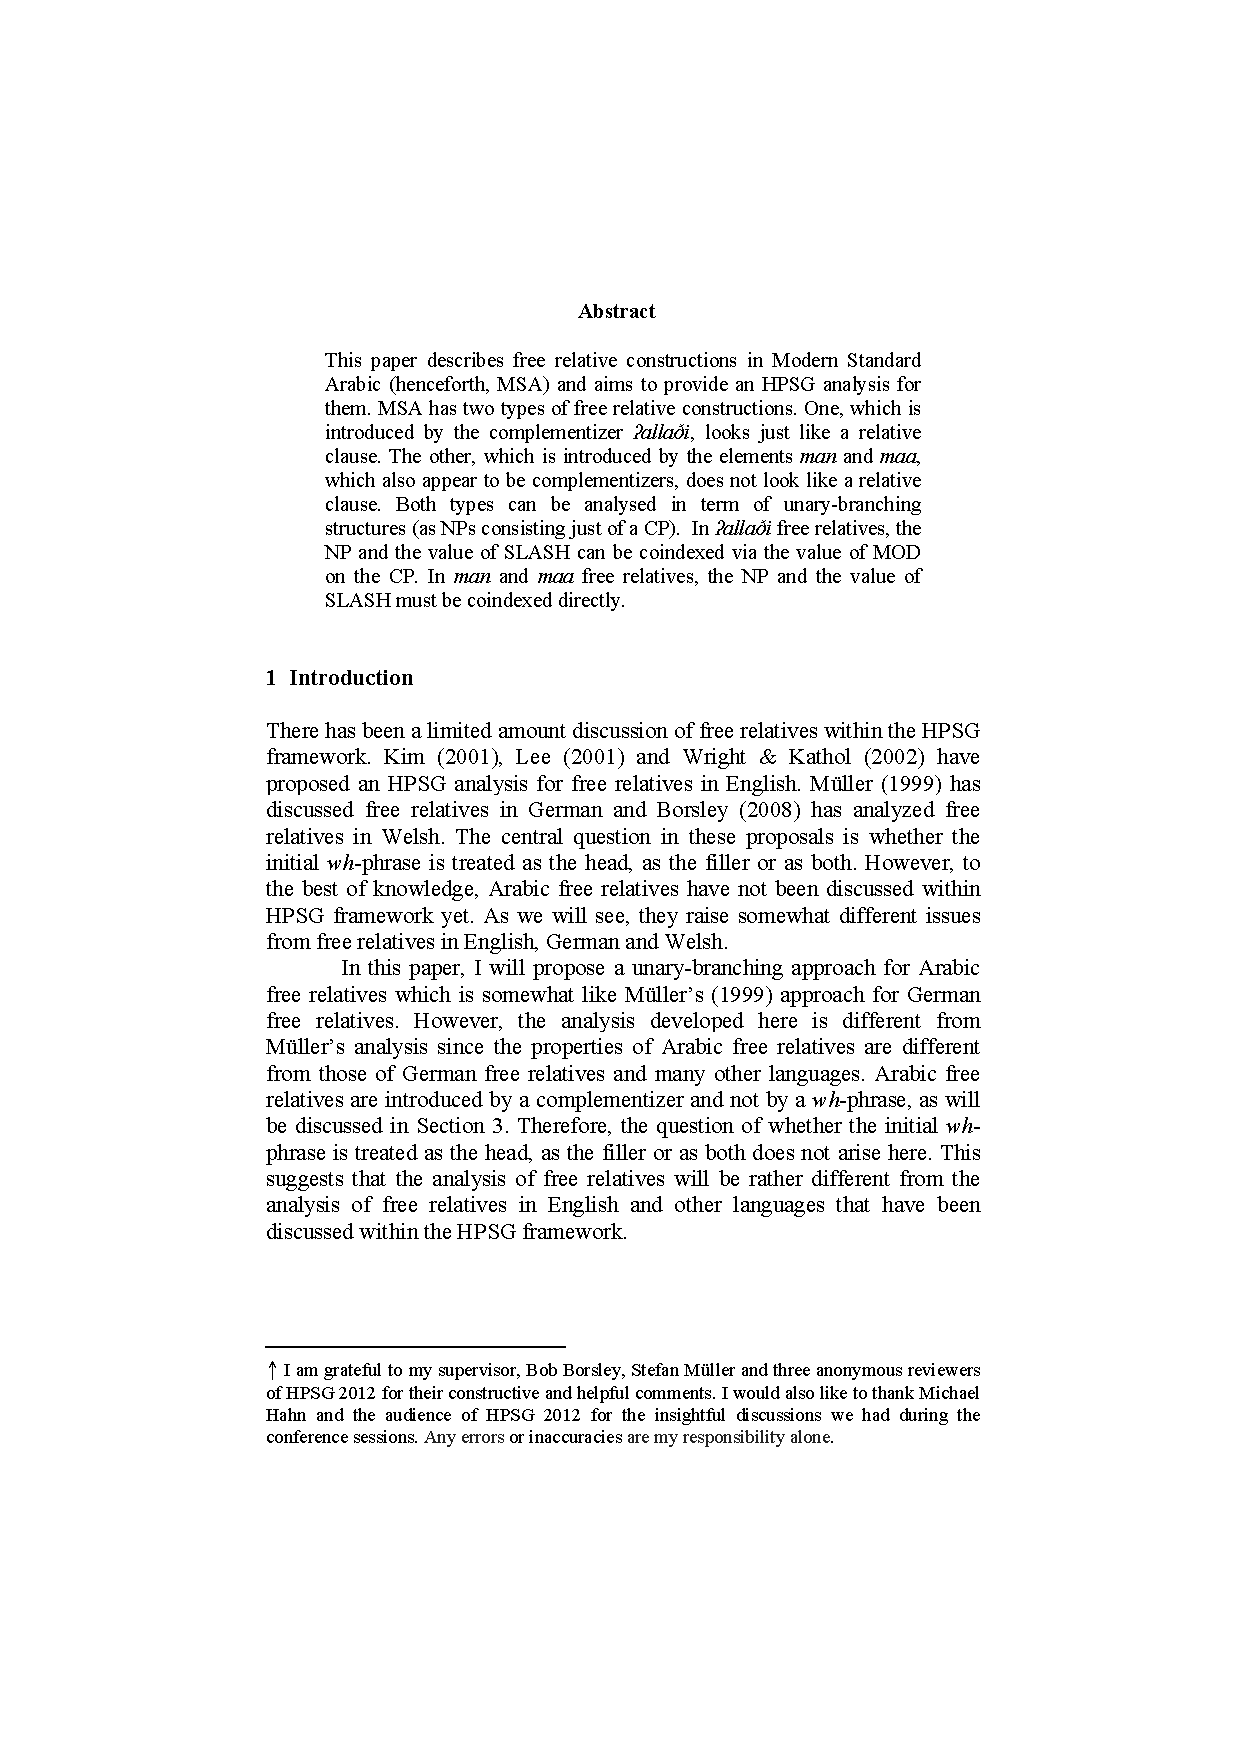
\includepdf[pages=-,pagecommand=\thispagestyle{plain}]{Includes/alqurashi.pdf}
        \setcounter{page}{26}
        \phantomsection
        \addcontentsline{toc}{section}{Abdulrahman Alqurashi, Robert D. Borsley: Arabic Relative Clauses in HPSG}
\thispagestyle{empty}

\begin{center}
  {\huge\bfseries Arabic Relative Clauses in HPSG\par}

  \bigskip

~\\
\begingroup
\setlength{\leftskip}{0pt plus 1fill}
\setlength{\rightskip}{0pt plus 1fill}
\setlength{\parindent}{0pt}
\setlength{\parfillskip}{0pt}
  \formatauthor{Abdulrahman Alqurashi}{\begin{tabular}{@{}c@{}}King Abdulaziz University, University of Essex\end{tabular}}
\formatauthor{Robert D. Borsley}{\begin{tabular}{@{}c@{}}University of Essex\end{tabular}}

\par\endgroup

  \vspace*{8ex}

  Proceedings of the 19th International Conference on\par Head-Driven Phrase Structure Grammar

  \bigskip

  Chungnam National University Daejeon

  \medskip

  Stefan Müller (Editor)

  \medskip

  2012

  \medskip

  CSLI Publications

  \medskip

  pages 26--44

  \medskip

  \url{http://csli-publications.stanford.edu/HPSG/2012}
\end{center}
\vfill

\noindent



\vfill
\noindent
% APA Style
Alqurashi, Abdulrahman, \& Borsley, Robert D. 2012. Arabic Relative Clauses in HPSG. In Müller, Stefan (Ed.), \emph{{Proceedings of the 19th International Conference on Head-Driven Phrase Structure Grammar, Chungnam National University Daejeon}}, 26--44. Stanford,
CA: CSLI Publications. \hfill\href{http://creativecommons.org/licenses/by/4.0/}{\includegraphics[height=.75em]{Includes/ccby.eps}}

\newpage
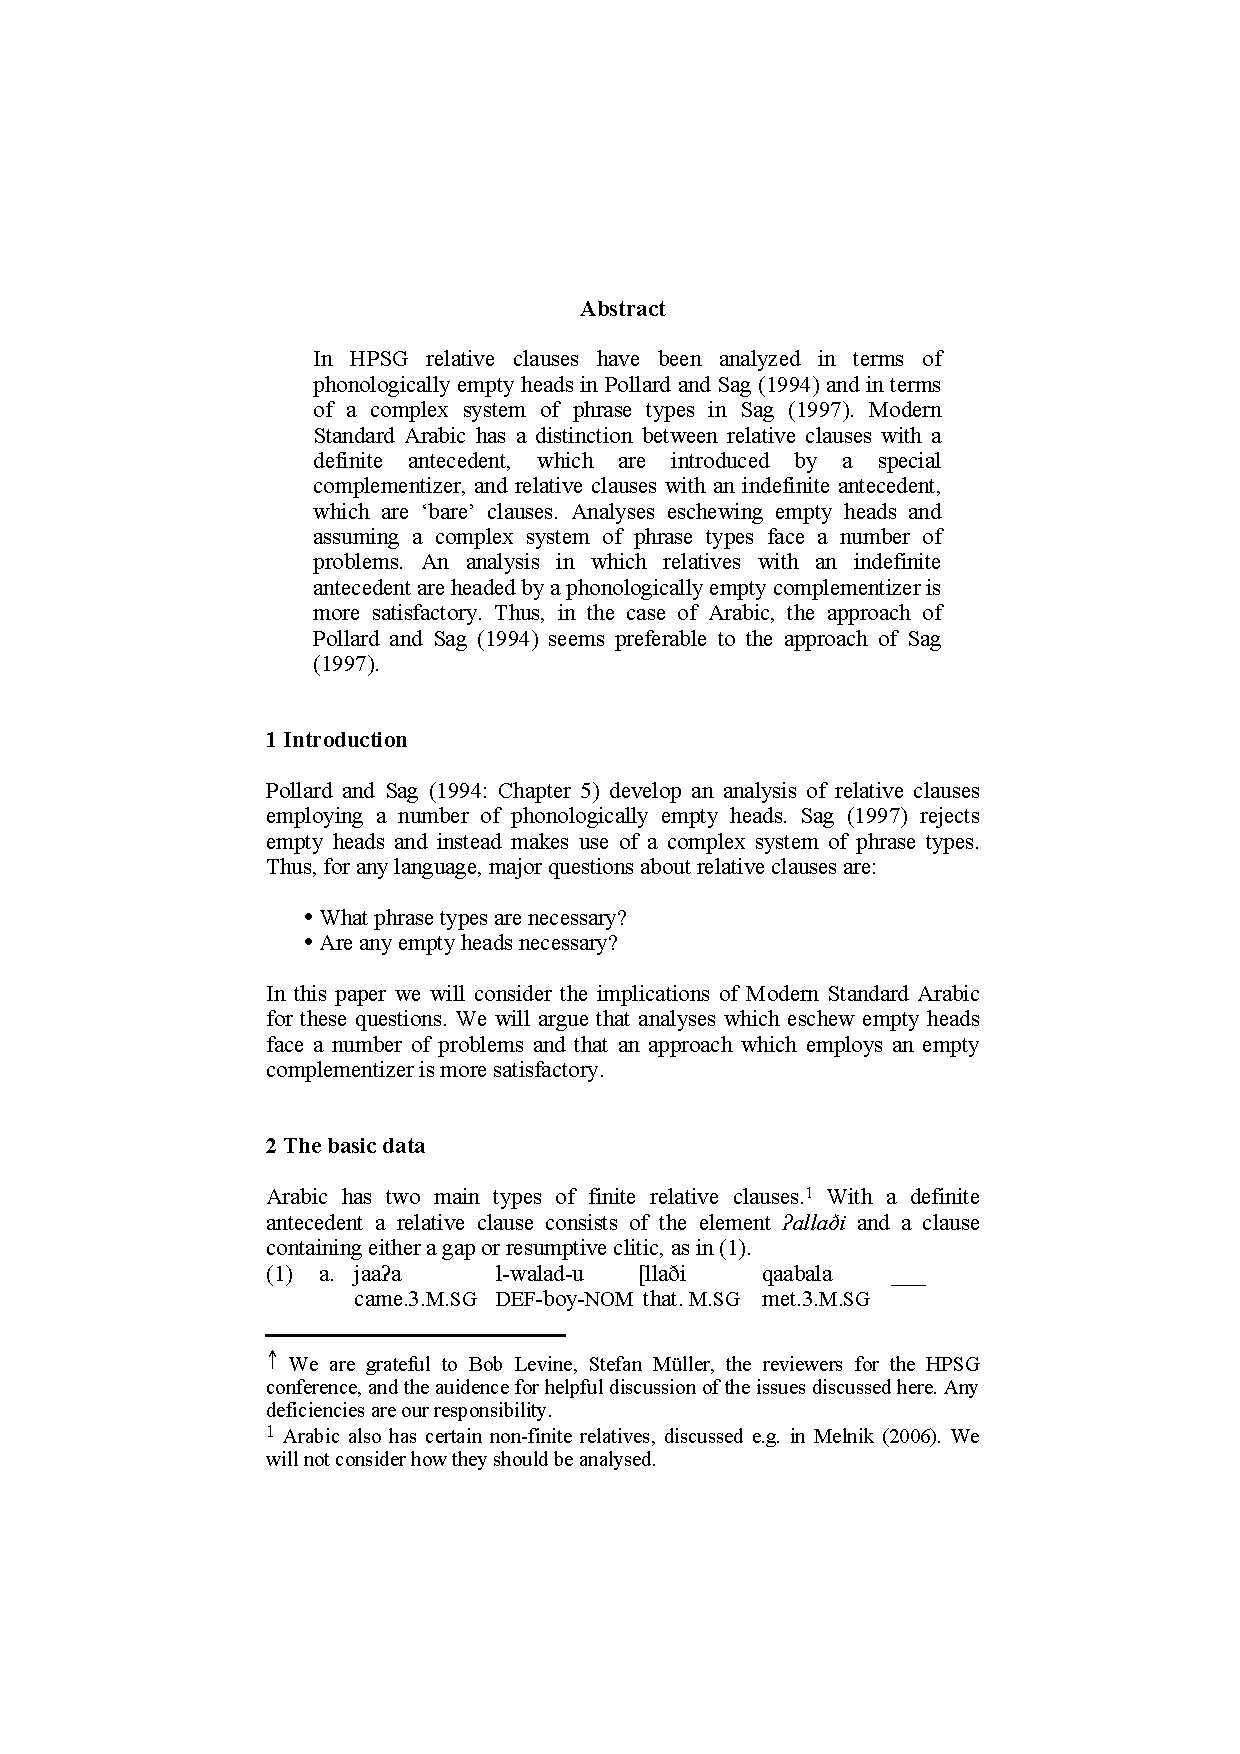
\includepdf[pages=-,pagecommand=\thispagestyle{plain}]{Includes/alqurashi-borsley.pdf}
        \setcounter{page}{45}
        \phantomsection
        \addcontentsline{toc}{section}{Anne Bjerre: An Analysis of Danish Free Relatives}
\thispagestyle{empty}

\begin{center}
  {\huge\bfseries An Analysis of Danish Free Relatives\par}

  \bigskip

~\\
\begingroup
\setlength{\leftskip}{0pt plus 1fill}
\setlength{\rightskip}{0pt plus 1fill}
\setlength{\parindent}{0pt}
\setlength{\parfillskip}{0pt}
  \formatauthor{Anne Bjerre}{\begin{tabular}{@{}c@{}}University of Southern Denmark\end{tabular}}

\par\endgroup

  \vspace*{8ex}

  Proceedings of the 19th International Conference on\par Head-Driven Phrase Structure Grammar

  \bigskip

  Chungnam National University Daejeon

  \medskip

  Stefan Müller (Editor)

  \medskip

  2012

  \medskip

  CSLI Publications

  \medskip

  pages 45--63

  \medskip

  \url{http://csli-publications.stanford.edu/HPSG/2012}
\end{center}
\vfill

\noindent



\vfill
\noindent
% APA Style
Bjerre, Anne. 2012. An Analysis of Danish Free Relatives. In Müller, Stefan (Ed.), \emph{{Proceedings of the 19th International Conference on Head-Driven Phrase Structure Grammar, Chungnam National University Daejeon}}, 45--63. Stanford,
CA: CSLI Publications. \hfill\href{http://creativecommons.org/licenses/by/4.0/}{\includegraphics[height=.75em]{Includes/ccby.eps}}

\newpage
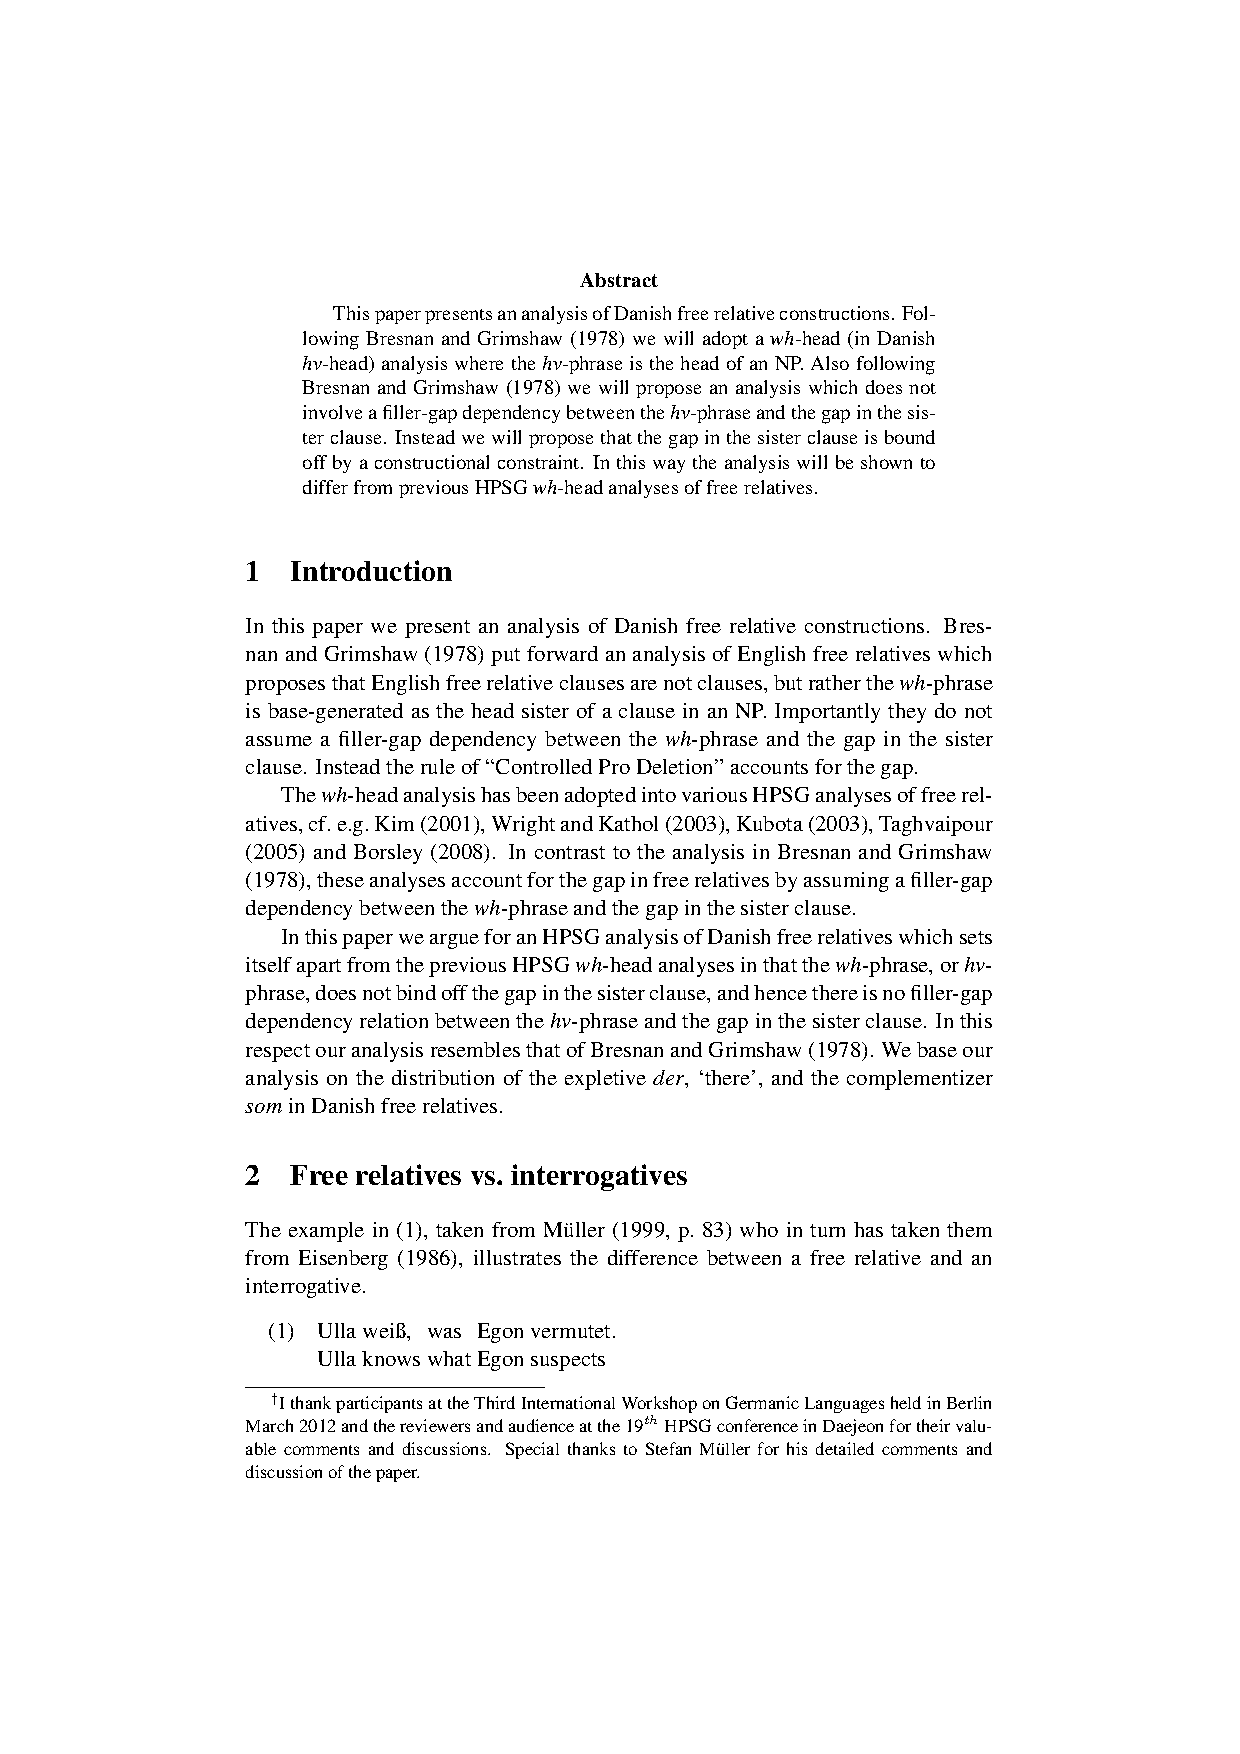
\includepdf[pages=-,pagecommand=\thispagestyle{plain}]{Includes/bjerre.pdf}
        \setcounter{page}{64}
        \phantomsection
        \addcontentsline{toc}{section}{Sae-Youn Cho, Na-Hyun Ku: Verbal Suffix-Repetition Construction in Korean: A Constraint- and Construction-based Approach}
\thispagestyle{empty}

\begin{center}
  {\huge\bfseries Verbal Suffix-Repetition Construction in Korean: A Constraint- and Construction-based Approach\par}

  \bigskip

~\\
\begingroup
\setlength{\leftskip}{0pt plus 1fill}
\setlength{\rightskip}{0pt plus 1fill}
\setlength{\parindent}{0pt}
\setlength{\parfillskip}{0pt}
  \formatauthor{Sae-Youn Cho}{\begin{tabular}{@{}c@{}}Kangwon National University\end{tabular}}
\formatauthor{Na-Hyun Ku}{\begin{tabular}{@{}c@{}}Kangwon National University\end{tabular}}

\par\endgroup

  \vspace*{8ex}

  Proceedings of the 19th International Conference on\par Head-Driven Phrase Structure Grammar

  \bigskip

  Chungnam National University Daejeon

  \medskip

  Stefan Müller (Editor)

  \medskip

  2012

  \medskip

  CSLI Publications

  \medskip

  pages 64--74

  \medskip

  \url{http://csli-publications.stanford.edu/HPSG/2012}
\end{center}
\vfill

\noindent



\vfill
\noindent
% APA Style
Cho, Sae-Youn, \& Ku, Na-Hyun. 2012. Verbal Suffix-Repetition Construction in Korean: A Constraint- and Construction-based Approach. In Müller, Stefan (Ed.), \emph{{Proceedings of the 19th International Conference on Head-Driven Phrase Structure Grammar, Chungnam National University Daejeon}}, 64--74. Stanford,
CA: CSLI Publications. \hfill\href{http://creativecommons.org/licenses/by/4.0/}{\includegraphics[height=.75em]{Includes/ccby.eps}}

\newpage
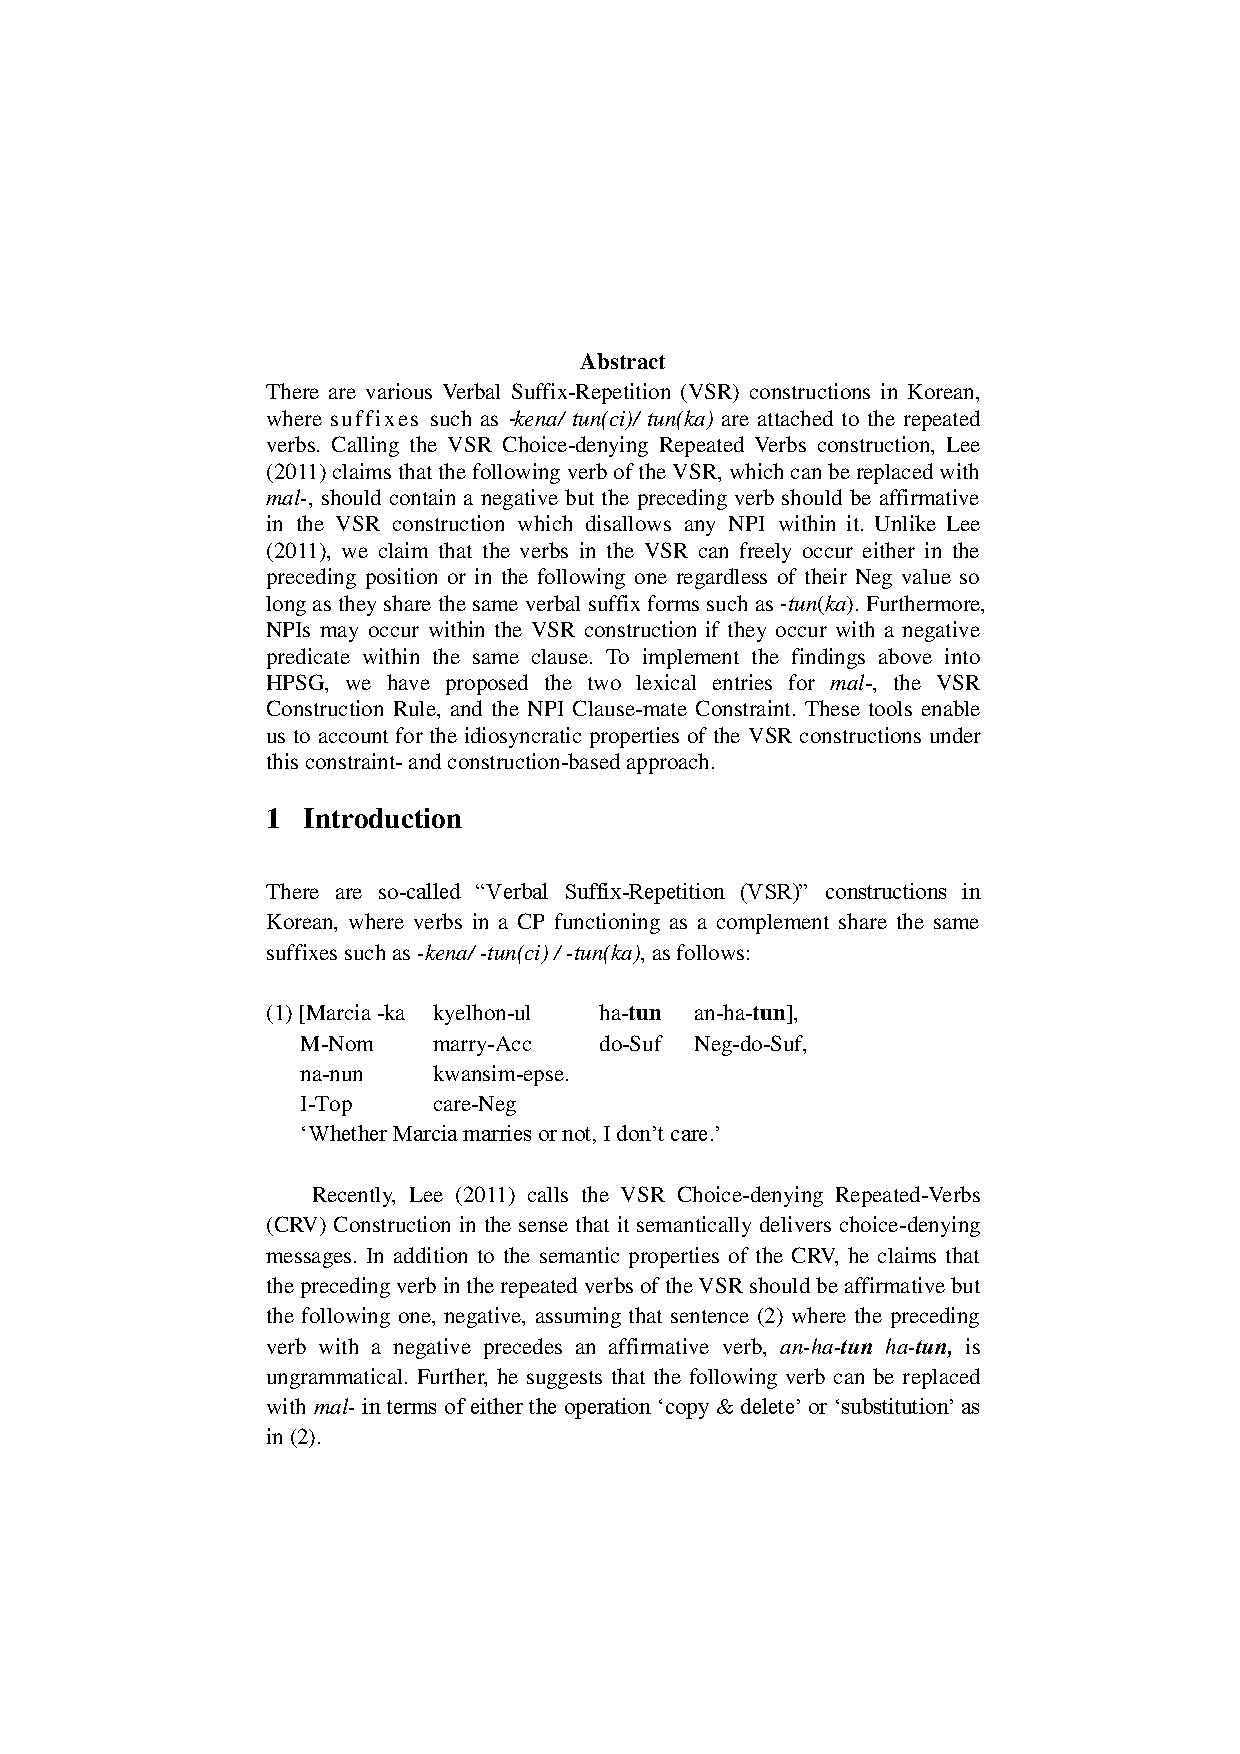
\includepdf[pages=-,pagecommand=\thispagestyle{plain}]{Includes/cho-ku.pdf}
        \setcounter{page}{75}
        \phantomsection
        \addcontentsline{toc}{section}{Incheol Choi: Sentential Specifiers in the Korean Clause Structure}
\thispagestyle{empty}

\begin{center}
  {\huge\bfseries Sentential Specifiers in the Korean Clause Structure\par}

  \bigskip

~\\
\begingroup
\setlength{\leftskip}{0pt plus 1fill}
\setlength{\rightskip}{0pt plus 1fill}
\setlength{\parindent}{0pt}
\setlength{\parfillskip}{0pt}
  \formatauthor{Incheol Choi}{\begin{tabular}{@{}c@{}}Kyungpook National University\end{tabular}}

\par\endgroup

  \vspace*{8ex}

  Proceedings of the 19th International Conference on\par Head-Driven Phrase Structure Grammar

  \bigskip

  Chungnam National University Daejeon

  \medskip

  Stefan Müller (Editor)

  \medskip

  2012

  \medskip

  CSLI Publications

  \medskip

  pages 75--85

  \medskip

  \url{http://csli-publications.stanford.edu/HPSG/2012}
\end{center}
\vfill

\noindent



\vfill
\noindent
% APA Style
Choi, Incheol. 2012. Sentential Specifiers in the Korean Clause Structure. In Müller, Stefan (Ed.), \emph{{Proceedings of the 19th International Conference on Head-Driven Phrase Structure Grammar, Chungnam National University Daejeon}}, 75--85. Stanford,
CA: CSLI Publications. \hfill\href{http://creativecommons.org/licenses/by/4.0/}{\includegraphics[height=.75em]{Includes/ccby.eps}}

\newpage
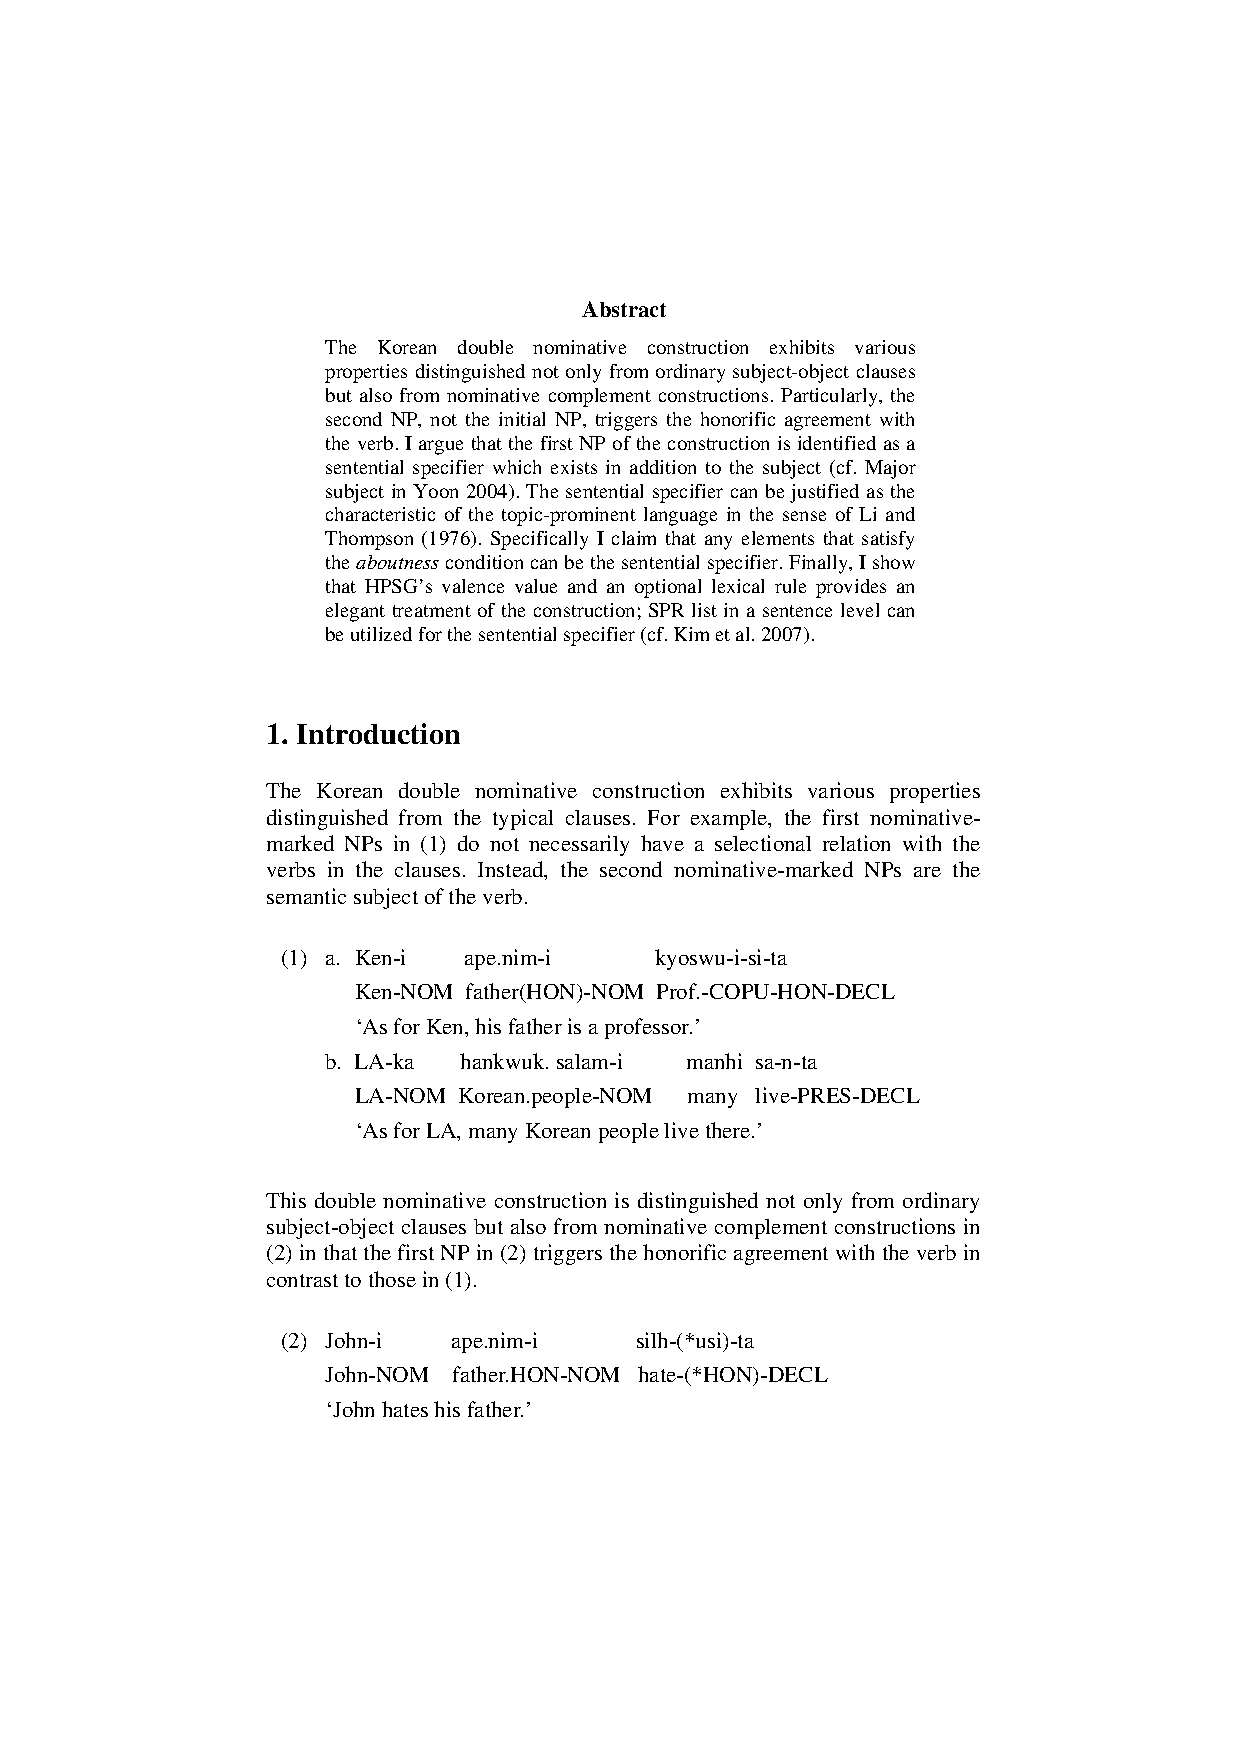
\includepdf[pages=-,pagecommand=\thispagestyle{plain}]{Includes/choi.pdf}
        \setcounter{page}{86}
        \phantomsection
        \addcontentsline{toc}{section}{Francisco Costa, Ant{\'o}nio Branco: Backshift and Tense Decomposition}
\thispagestyle{empty}

\begin{center}
  {\huge\bfseries Backshift and Tense Decomposition\par}

  \bigskip

~\\
\begingroup
\setlength{\leftskip}{0pt plus 1fill}
\setlength{\rightskip}{0pt plus 1fill}
\setlength{\parindent}{0pt}
\setlength{\parfillskip}{0pt}
  \formatauthor{Francisco Costa}{\begin{tabular}{@{}c@{}}University of Lisbon\end{tabular}}
\formatauthor{António Branco}{\begin{tabular}{@{}c@{}}University of Lisbon\end{tabular}}

\par\endgroup

  \vspace*{8ex}

  Proceedings of the 19th International Conference on\par Head-Driven Phrase Structure Grammar

  \bigskip

  Chungnam National University Daejeon

  \medskip

  Stefan Müller (Editor)

  \medskip

  2012

  \medskip

  CSLI Publications

  \medskip

  pages 86--106

  \medskip

  \url{http://csli-publications.stanford.edu/HPSG/2012}
\end{center}
\vfill

\noindent



\vfill
\noindent
% APA Style
Costa, Francisco, \& Branco, António. 2012. Backshift and Tense Decomposition. In Müller, Stefan (Ed.), \emph{{Proceedings of the 19th International Conference on Head-Driven Phrase Structure Grammar, Chungnam National University Daejeon}}, 86--106. Stanford,
CA: CSLI Publications. \hfill\href{http://creativecommons.org/licenses/by/4.0/}{\includegraphics[height=.75em]{Includes/ccby.eps}}

\newpage
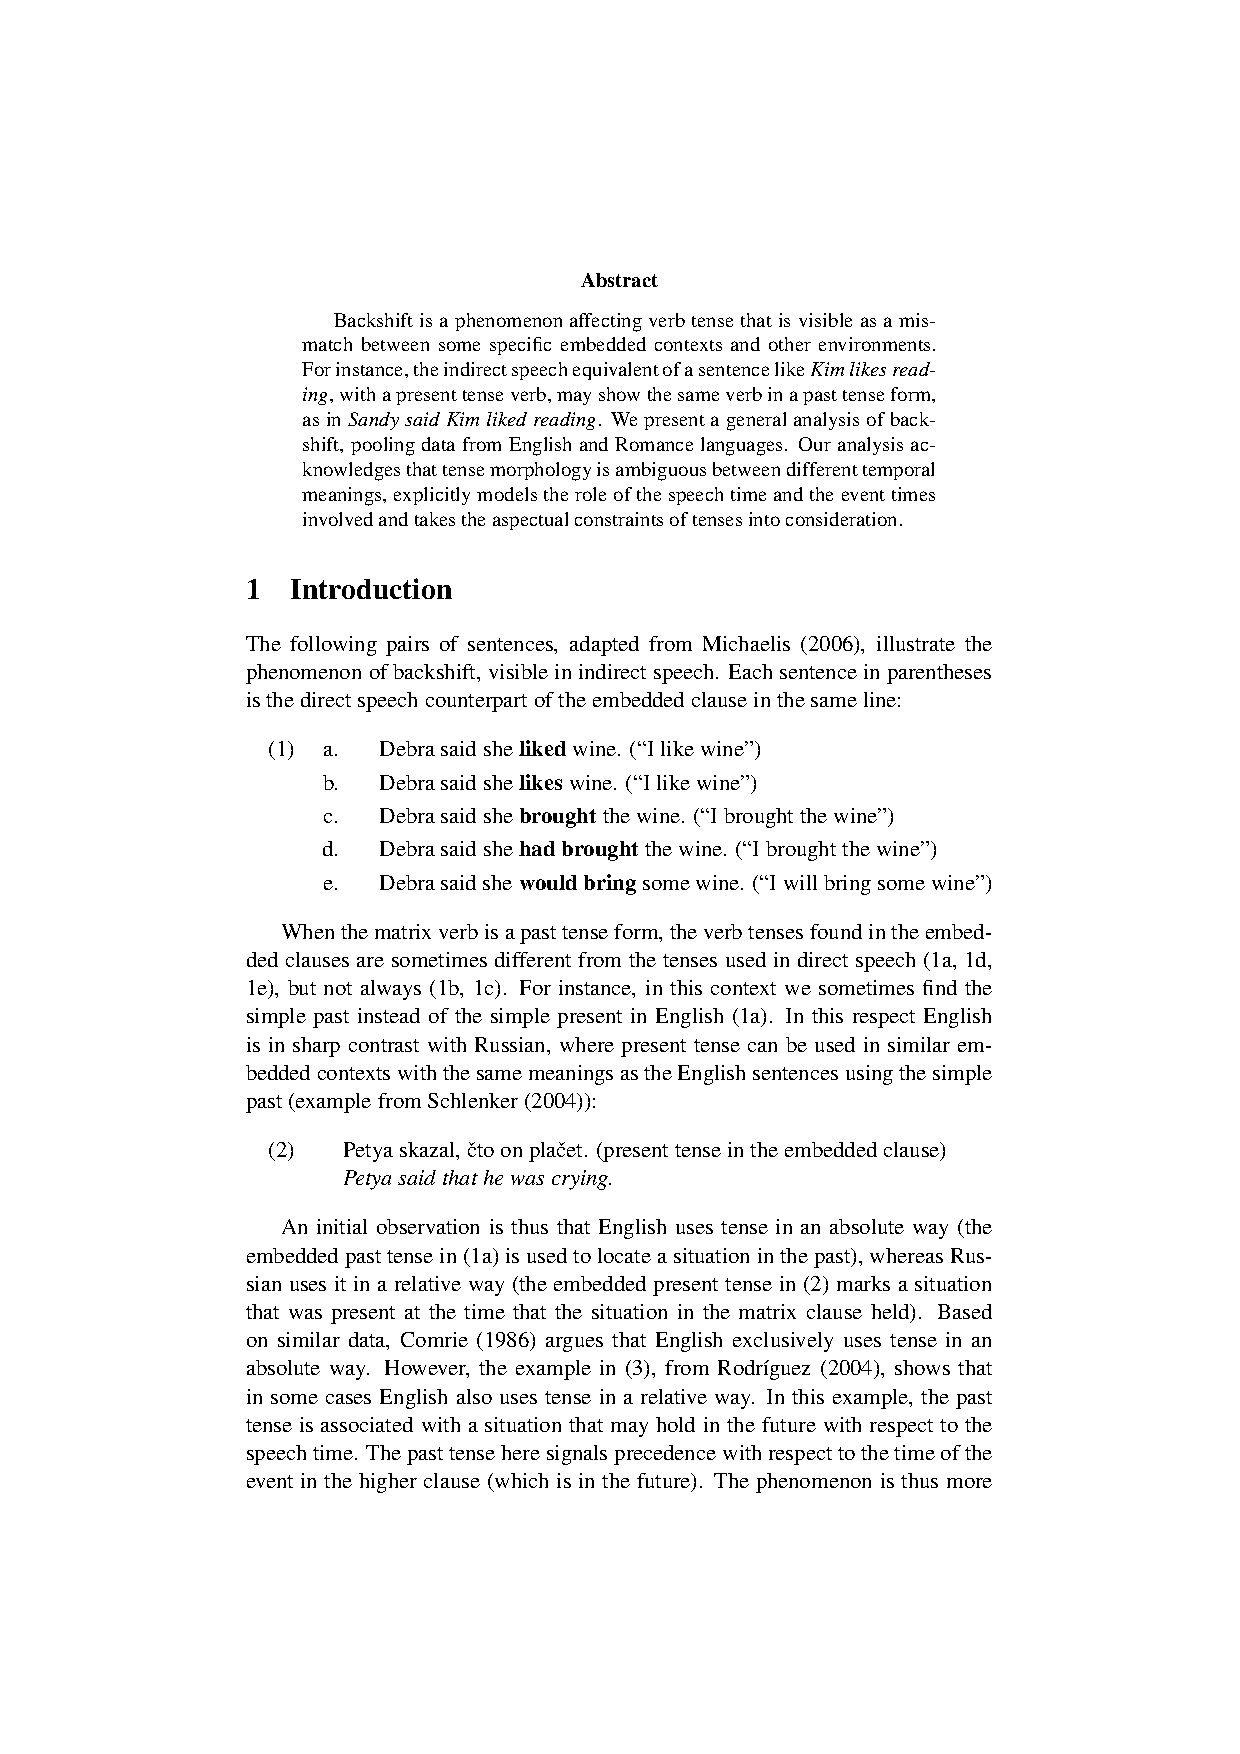
\includepdf[pages=-,pagecommand=\thispagestyle{plain}]{Includes/costa-branco.pdf}
        \setcounter{page}{107}
        \phantomsection
        \addcontentsline{toc}{section}{Joshua Crowgey: An a priori Typology of Sentential Negation from an HPSG Perspective}
\thispagestyle{empty}

\begin{center}
  {\huge\bfseries An a priori Typology of Sentential Negation from an HPSG Perspective\par}

  \bigskip

~\\
\begingroup
\setlength{\leftskip}{0pt plus 1fill}
\setlength{\rightskip}{0pt plus 1fill}
\setlength{\parindent}{0pt}
\setlength{\parfillskip}{0pt}
  \formatauthor{Joshua Crowgey}{\begin{tabular}{@{}c@{}}University of Washington\end{tabular}}

\par\endgroup

  \vspace*{8ex}

  Proceedings of the 19th International Conference on\par Head-Driven Phrase Structure Grammar

  \bigskip

  Chungnam National University Daejeon

  \medskip

  Stefan Müller (Editor)

  \medskip

  2012

  \medskip

  CSLI Publications

  \medskip

  pages 107--122

  \medskip

  \url{http://csli-publications.stanford.edu/HPSG/2012}
\end{center}
\vfill

\noindent



\vfill
\noindent
% APA Style
Crowgey, Joshua. 2012. An a priori Typology of Sentential Negation from an HPSG Perspective. In Müller, Stefan (Ed.), \emph{{Proceedings of the 19th International Conference on Head-Driven Phrase Structure Grammar, Chungnam National University Daejeon}}, 107--122. Stanford,
CA: CSLI Publications. \hfill\href{http://creativecommons.org/licenses/by/4.0/}{\includegraphics[height=.75em]{Includes/ccby.eps}}

\newpage
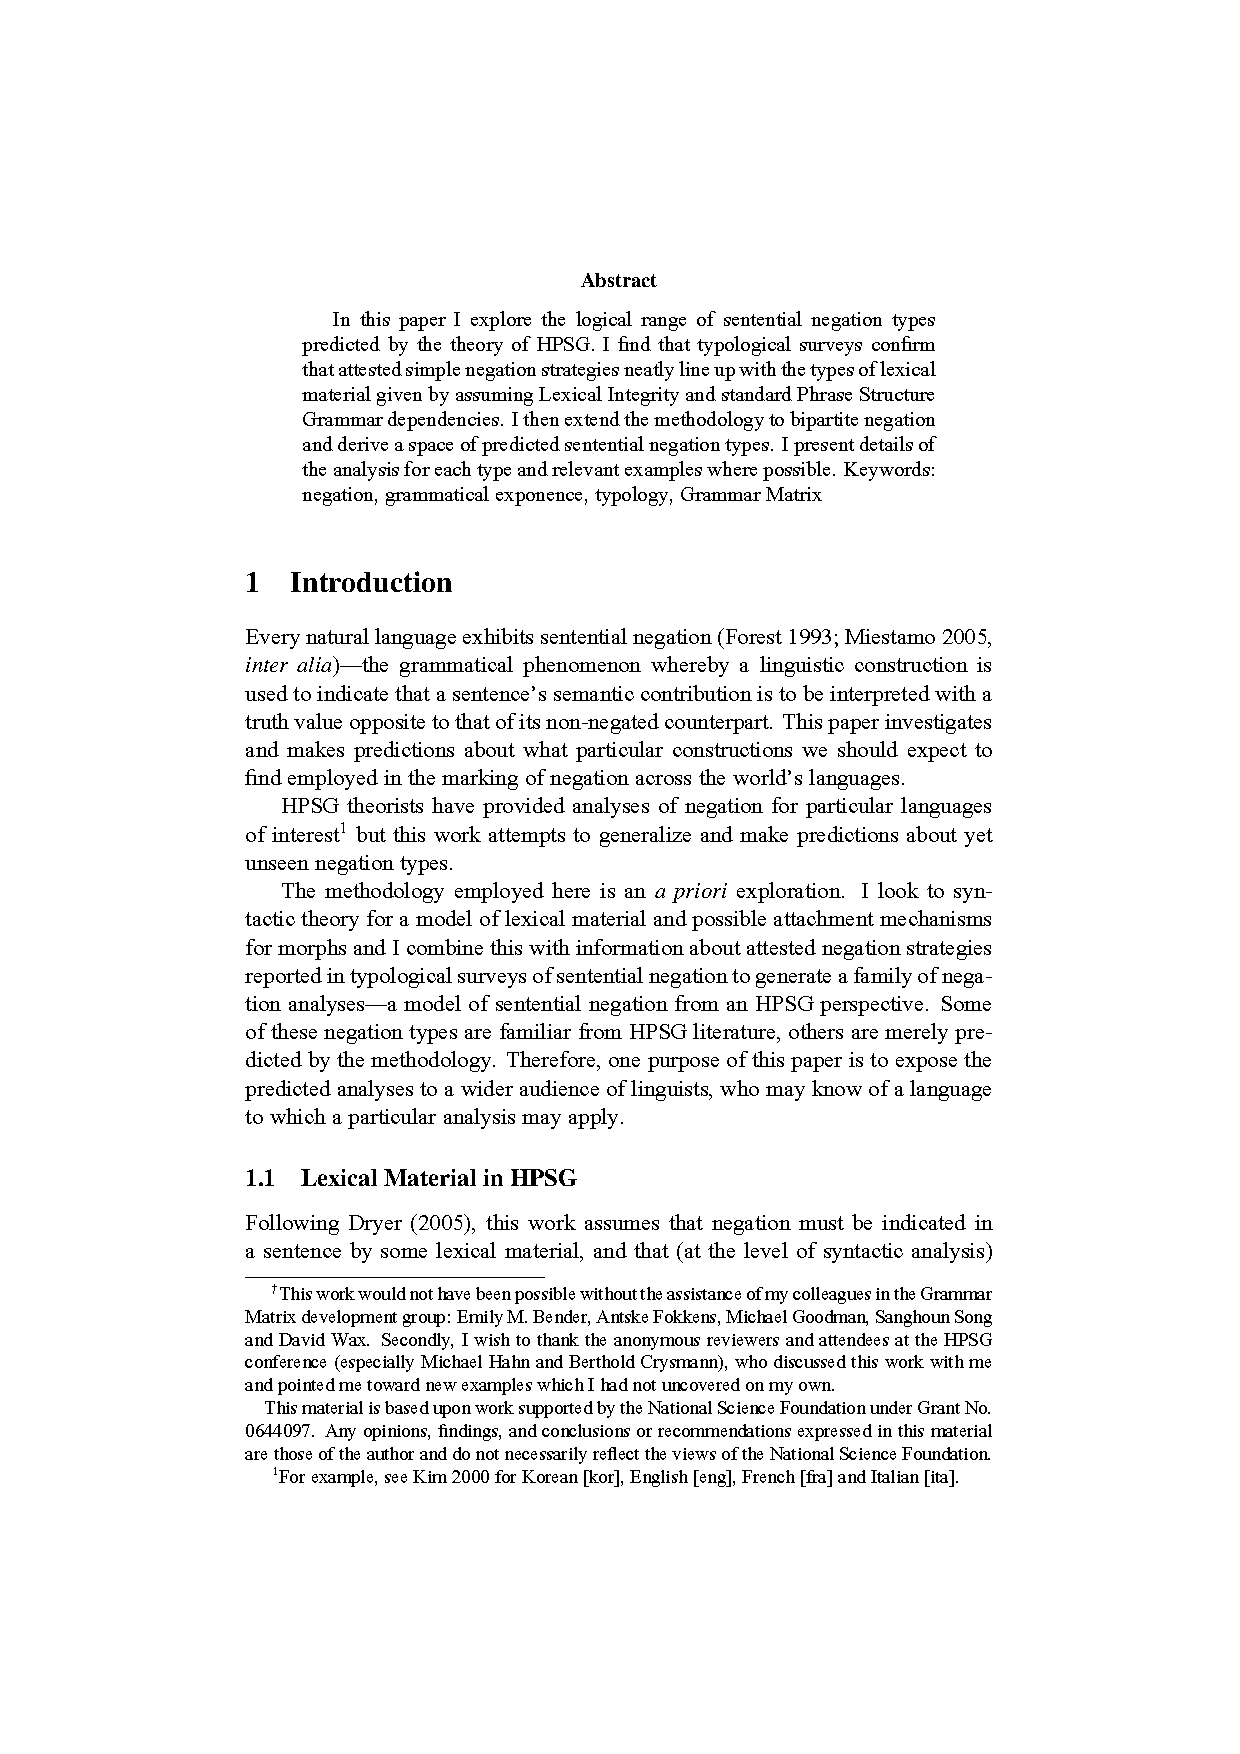
\includepdf[pages=-,pagecommand=\thispagestyle{plain}]{Includes/crowgey.pdf}
        \setcounter{page}{123}
        \phantomsection
        \addcontentsline{toc}{section}{Berthold Crysmann, Olivier Bonami: Establishing Order in Type-Based Realisational Morphology}
\thispagestyle{empty}

\begin{center}
  {\huge\bfseries Establishing Order in Type-Based Realisational Morphology\par}

  \bigskip

~\\
\begingroup
\setlength{\leftskip}{0pt plus 1fill}
\setlength{\rightskip}{0pt plus 1fill}
\setlength{\parindent}{0pt}
\setlength{\parfillskip}{0pt}
  \formatauthor{Berthold Crysmann}{\begin{tabular}{@{}c@{}}Laboratoire de Linguistique Formelle, Université Paris Diderot and CNRS\end{tabular}}
\formatauthor{Olivier Bonami}{\begin{tabular}{@{}c@{}}Université Paris-Sorbonne, Institut Universitaire de France, Laboratoire de Linguistique Formelle\end{tabular}}

\par\endgroup

  \vspace*{8ex}

  Proceedings of the 19th International Conference on\par Head-Driven Phrase Structure Grammar

  \bigskip

  Chungnam National University Daejeon

  \medskip

  Stefan Müller (Editor)

  \medskip

  2012

  \medskip

  CSLI Publications

  \medskip

  pages 123--143

  \medskip

  \url{http://csli-publications.stanford.edu/HPSG/2012}
\end{center}
\vfill

\noindent



\vfill
\noindent
% APA Style
Crysmann, Berthold, \& Bonami, Olivier. 2012. Establishing Order in Type-Based Realisational Morphology. In Müller, Stefan (Ed.), \emph{{Proceedings of the 19th International Conference on Head-Driven Phrase Structure Grammar, Chungnam National University Daejeon}}, 123--143. Stanford,
CA: CSLI Publications. \hfill\href{http://creativecommons.org/licenses/by/4.0/}{\includegraphics[height=.75em]{Includes/ccby.eps}}

\newpage
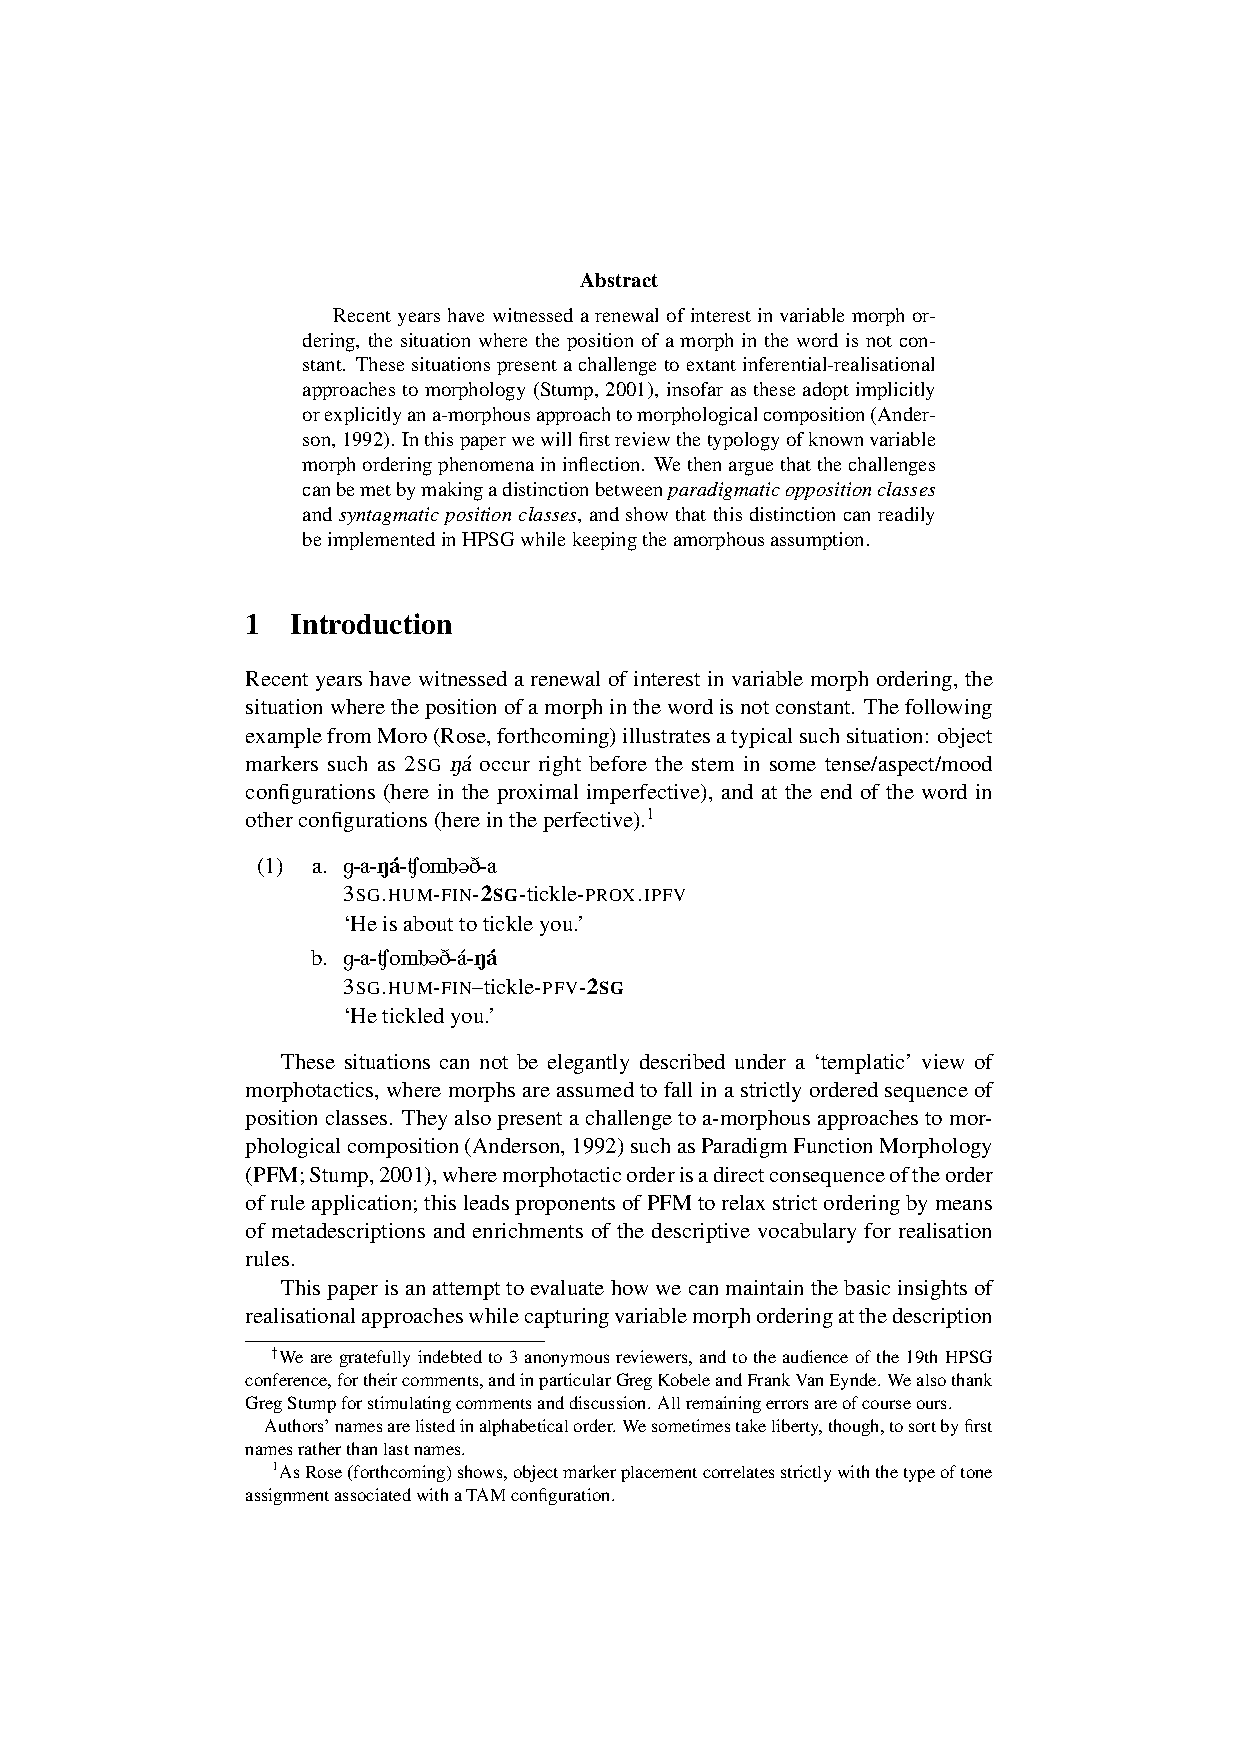
\includepdf[pages=-,pagecommand=\thispagestyle{plain}]{Includes/crysmann-bonami.pdf}
        \setcounter{page}{144}
        \phantomsection
        \addcontentsline{toc}{section}{Michael Hahn: Arabic Relativization Patterns:\\ A Unified HPSG Analysis}
\thispagestyle{empty}

\begin{center}
  {\huge\bfseries Arabic Relativization Patterns:\par A Unified HPSG Analysis\par}

  \bigskip

~\\
\begingroup
\setlength{\leftskip}{0pt plus 1fill}
\setlength{\rightskip}{0pt plus 1fill}
\setlength{\parindent}{0pt}
\setlength{\parfillskip}{0pt}
  \formatauthor{Michael Hahn}{\begin{tabular}{@{}c@{}}University of Tübingen\end{tabular}}

\par\endgroup

  \vspace*{8ex}

  Proceedings of the 19th International Conference on\par Head-Driven Phrase Structure Grammar

  \bigskip

  Chungnam National University Daejeon

  \medskip

  Stefan Müller (Editor)

  \medskip

  2012

  \medskip

  CSLI Publications

  \medskip

  pages 144--164

  \medskip

  \url{http://csli-publications.stanford.edu/HPSG/2012}
\end{center}
\vfill

\noindent



\vfill
\noindent
% APA Style
Hahn, Michael. 2012. Arabic Relativization Patterns:  A Unified HPSG Analysis. In Müller, Stefan (Ed.), \emph{{Proceedings of the 19th International Conference on Head-Driven Phrase Structure Grammar, Chungnam National University Daejeon}}, 144--164. Stanford,
CA: CSLI Publications. \hfill\href{http://creativecommons.org/licenses/by/4.0/}{\includegraphics[height=.75em]{Includes/ccby.eps}}

\newpage
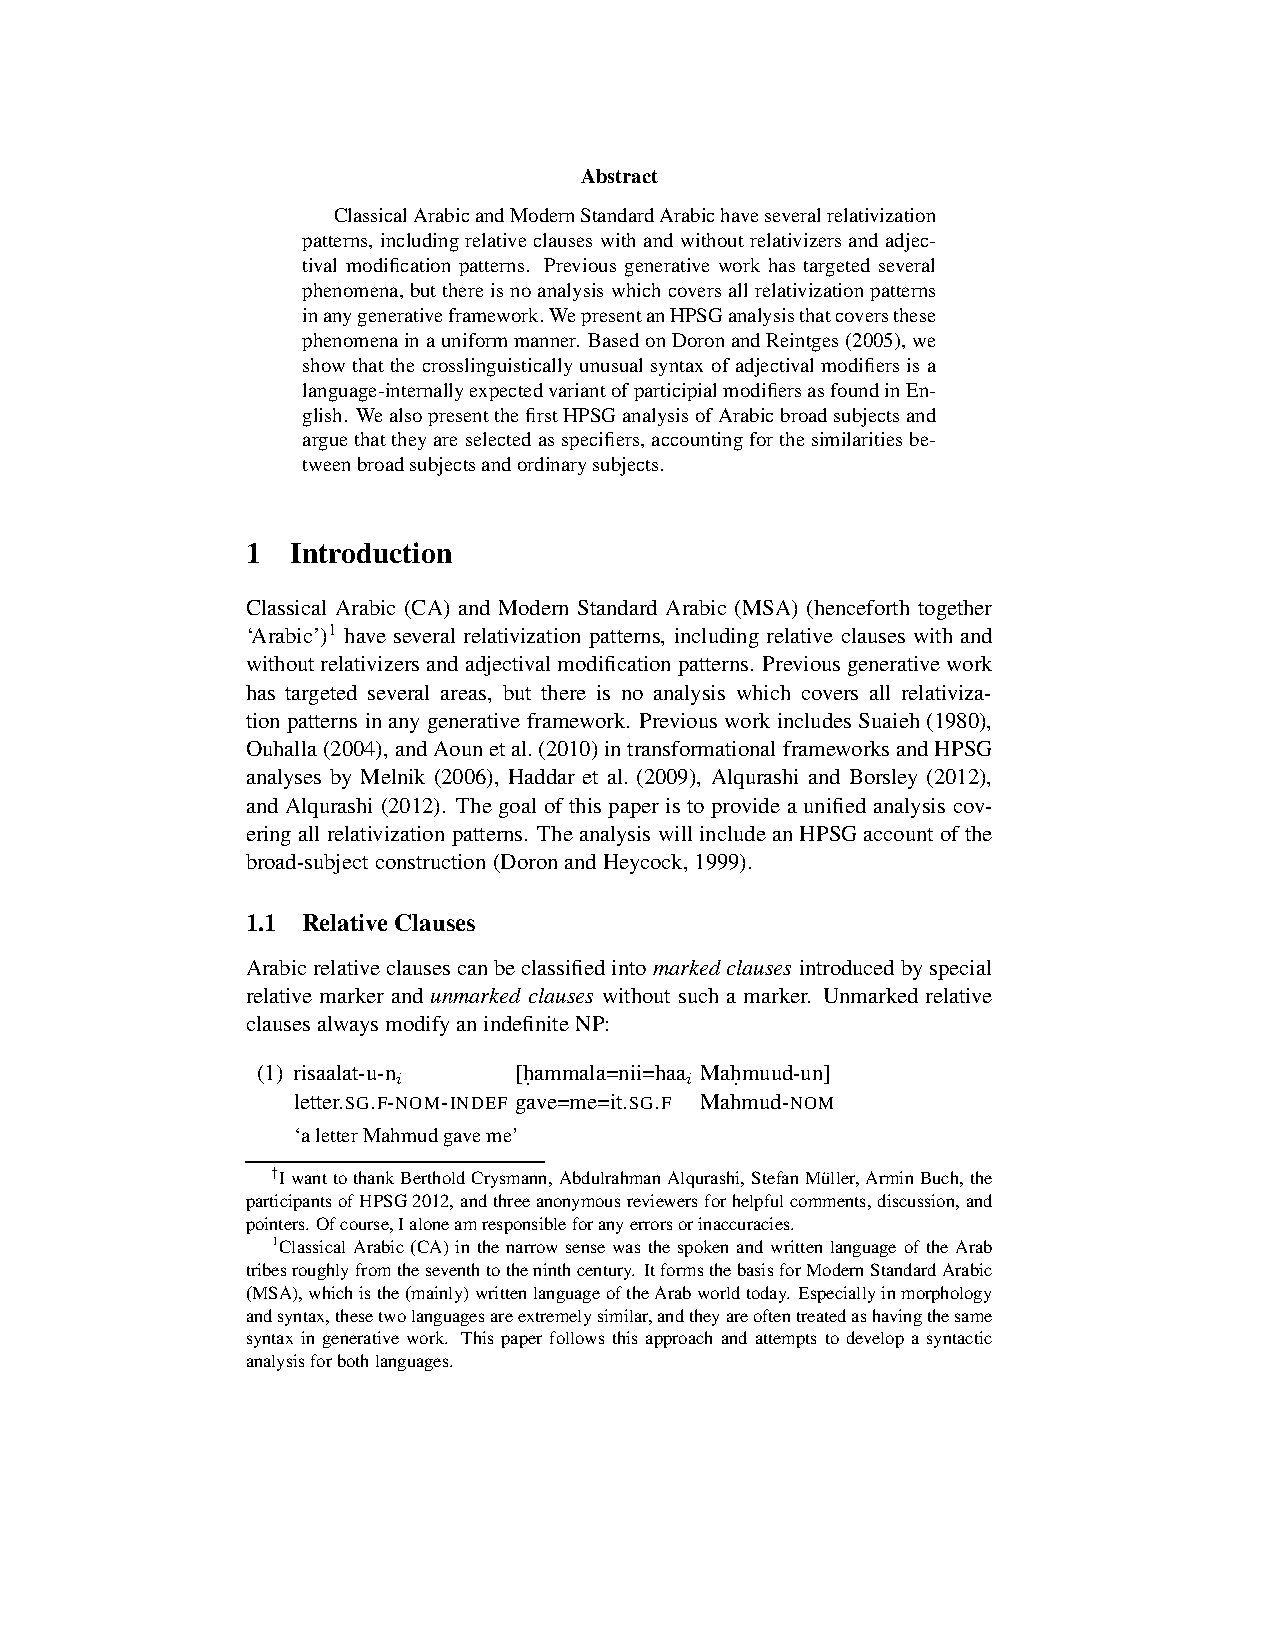
\includepdf[pages=-,pagecommand=\thispagestyle{plain}]{Includes/hahn.pdf}
        \setcounter{page}{165}
        \phantomsection
        \addcontentsline{toc}{section}{Petter Haugereid: The Adverb Argument Intersection Field in a Left-Branching Grammar of Norwegian}
\thispagestyle{empty}

\begin{center}
  {\huge\bfseries The Adverb Argument Intersection Field in a Left-Branching Grammar of Norwegian\par}

  \bigskip

~\\
\begingroup
\setlength{\leftskip}{0pt plus 1fill}
\setlength{\rightskip}{0pt plus 1fill}
\setlength{\parindent}{0pt}
\setlength{\parfillskip}{0pt}
  \formatauthor{Petter Haugereid}{\begin{tabular}{@{}c@{}}Nanyang Technological University, Singapore and University of Haifa, Israel\end{tabular}}

\par\endgroup

  \vspace*{8ex}

  Proceedings of the 19th International Conference on\par Head-Driven Phrase Structure Grammar

  \bigskip

  Chungnam National University Daejeon

  \medskip

  Stefan Müller (Editor)

  \medskip

  2012

  \medskip

  CSLI Publications

  \medskip

  pages 165--180

  \medskip

  \url{http://csli-publications.stanford.edu/HPSG/2012}
\end{center}
\vfill

\noindent



\vfill
\noindent
% APA Style
Haugereid, Petter. 2012. The Adverb Argument Intersection Field in a Left-Branching Grammar of Norwegian. In Müller, Stefan (Ed.), \emph{{Proceedings of the 19th International Conference on Head-Driven Phrase Structure Grammar, Chungnam National University Daejeon}}, 165--180. Stanford,
CA: CSLI Publications. \hfill\href{http://creativecommons.org/licenses/by/4.0/}{\includegraphics[height=.75em]{Includes/ccby.eps}}

\newpage
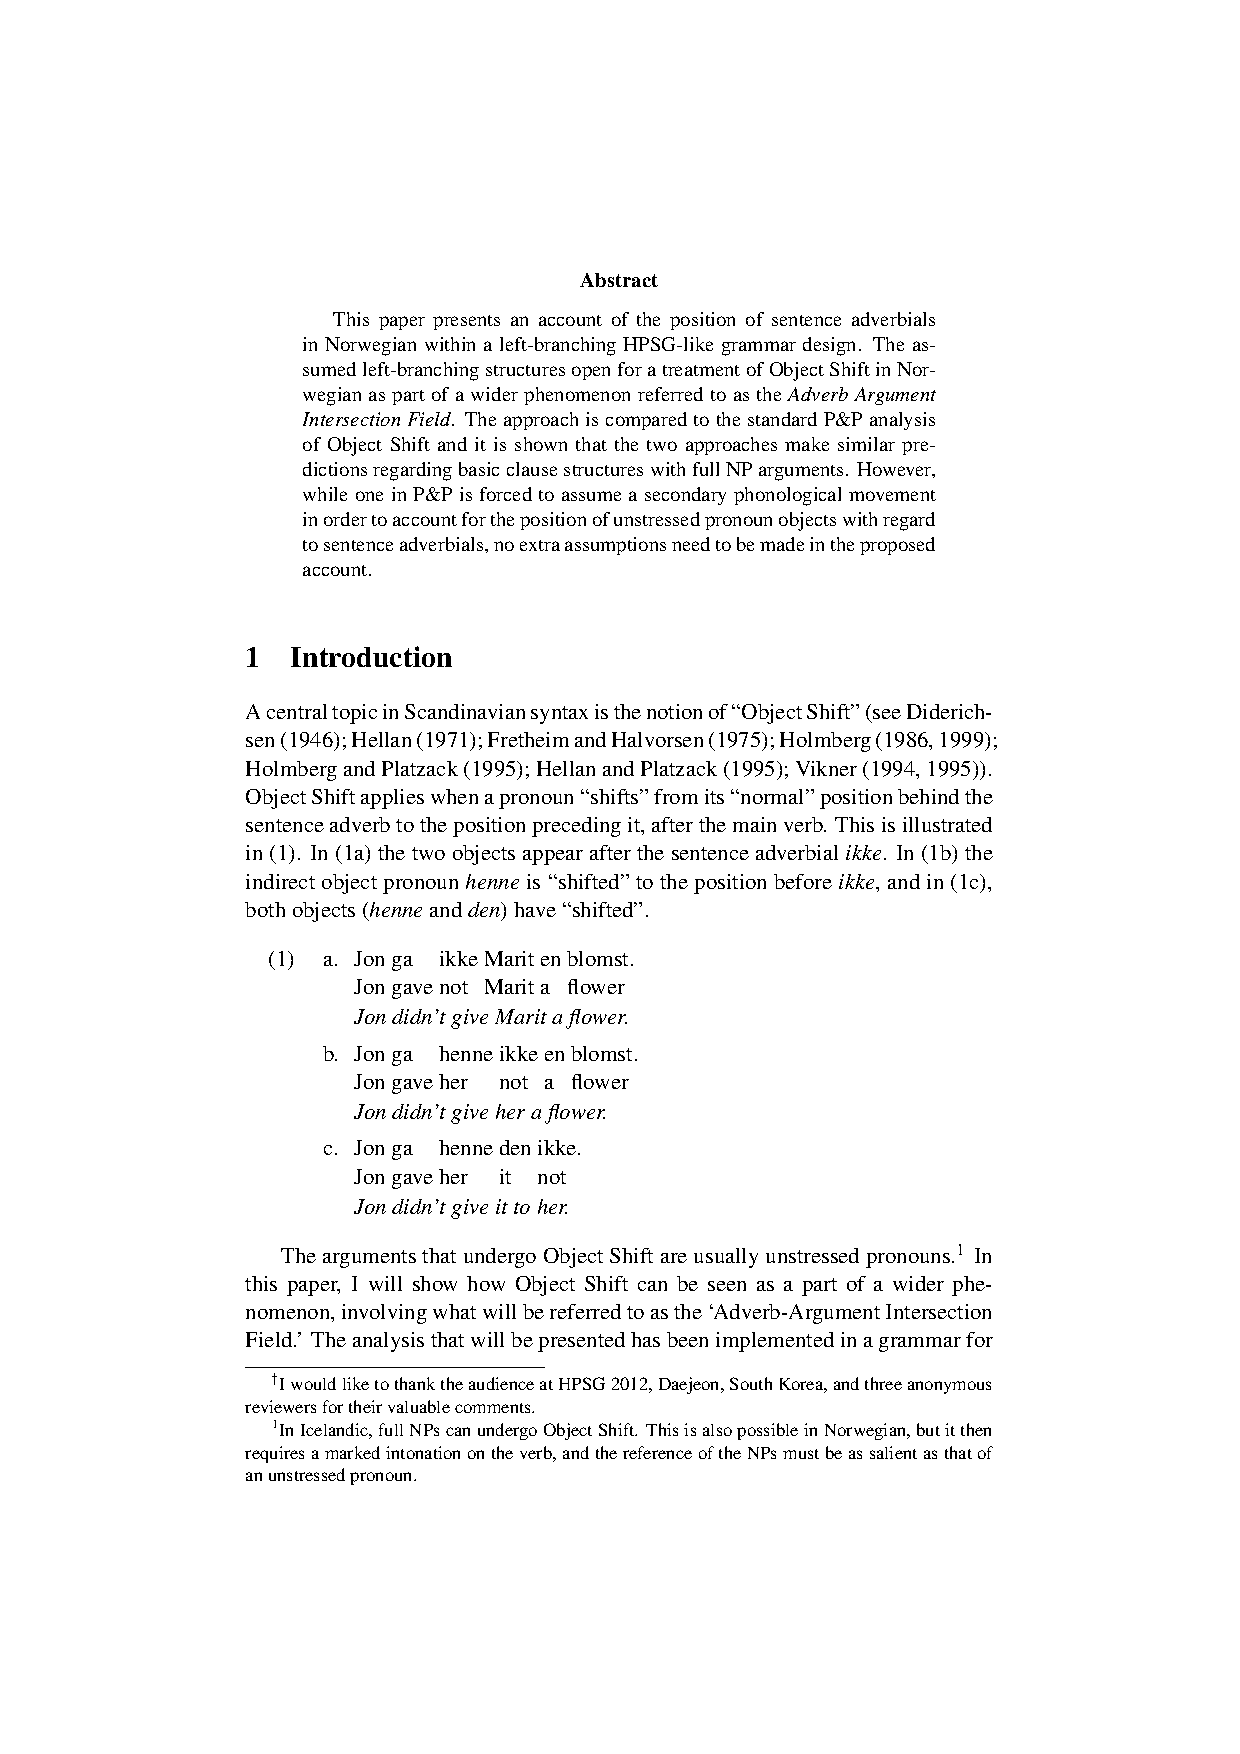
\includepdf[pages=-,pagecommand=\thispagestyle{plain}]{Includes/haugereid.pdf}
        \setcounter{page}{181}
        \phantomsection
        \addcontentsline{toc}{section}{Petter Haugereid, Mathieu Morey: A Left-Branching Grammar Design for Incremental Parsing}
\thispagestyle{empty}

\begin{center}
  {\huge\bfseries A Left-Branching Grammar Design for Incremental Parsing\par}

  \bigskip

~\\
\begingroup
\setlength{\leftskip}{0pt plus 1fill}
\setlength{\rightskip}{0pt plus 1fill}
\setlength{\parindent}{0pt}
\setlength{\parfillskip}{0pt}
  \formatauthor{Petter Haugereid}{\begin{tabular}{@{}c@{}}Nanyang Technological University, Singapore and University of Haifa, Israel\end{tabular}}
\formatauthor{Mathieu Morey}{\begin{tabular}{@{}c@{}}Aix-Marseille Université, France\end{tabular}}

\par\endgroup

  \vspace*{8ex}

  Proceedings of the 19th International Conference on\par Head-Driven Phrase Structure Grammar

  \bigskip

  Chungnam National University Daejeon

  \medskip

  Stefan Müller (Editor)

  \medskip

  2012

  \medskip

  CSLI Publications

  \medskip

  pages 181--194

  \medskip

  \url{http://csli-publications.stanford.edu/HPSG/2012}
\end{center}
\vfill

\noindent



\vfill
\noindent
% APA Style
Haugereid, Petter, \& Morey, Mathieu. 2012. A Left-Branching Grammar Design for Incremental Parsing. In Müller, Stefan (Ed.), \emph{{Proceedings of the 19th International Conference on Head-Driven Phrase Structure Grammar, Chungnam National University Daejeon}}, 181--194. Stanford,
CA: CSLI Publications. \hfill\href{http://creativecommons.org/licenses/by/4.0/}{\includegraphics[height=.75em]{Includes/ccby.eps}}

\newpage
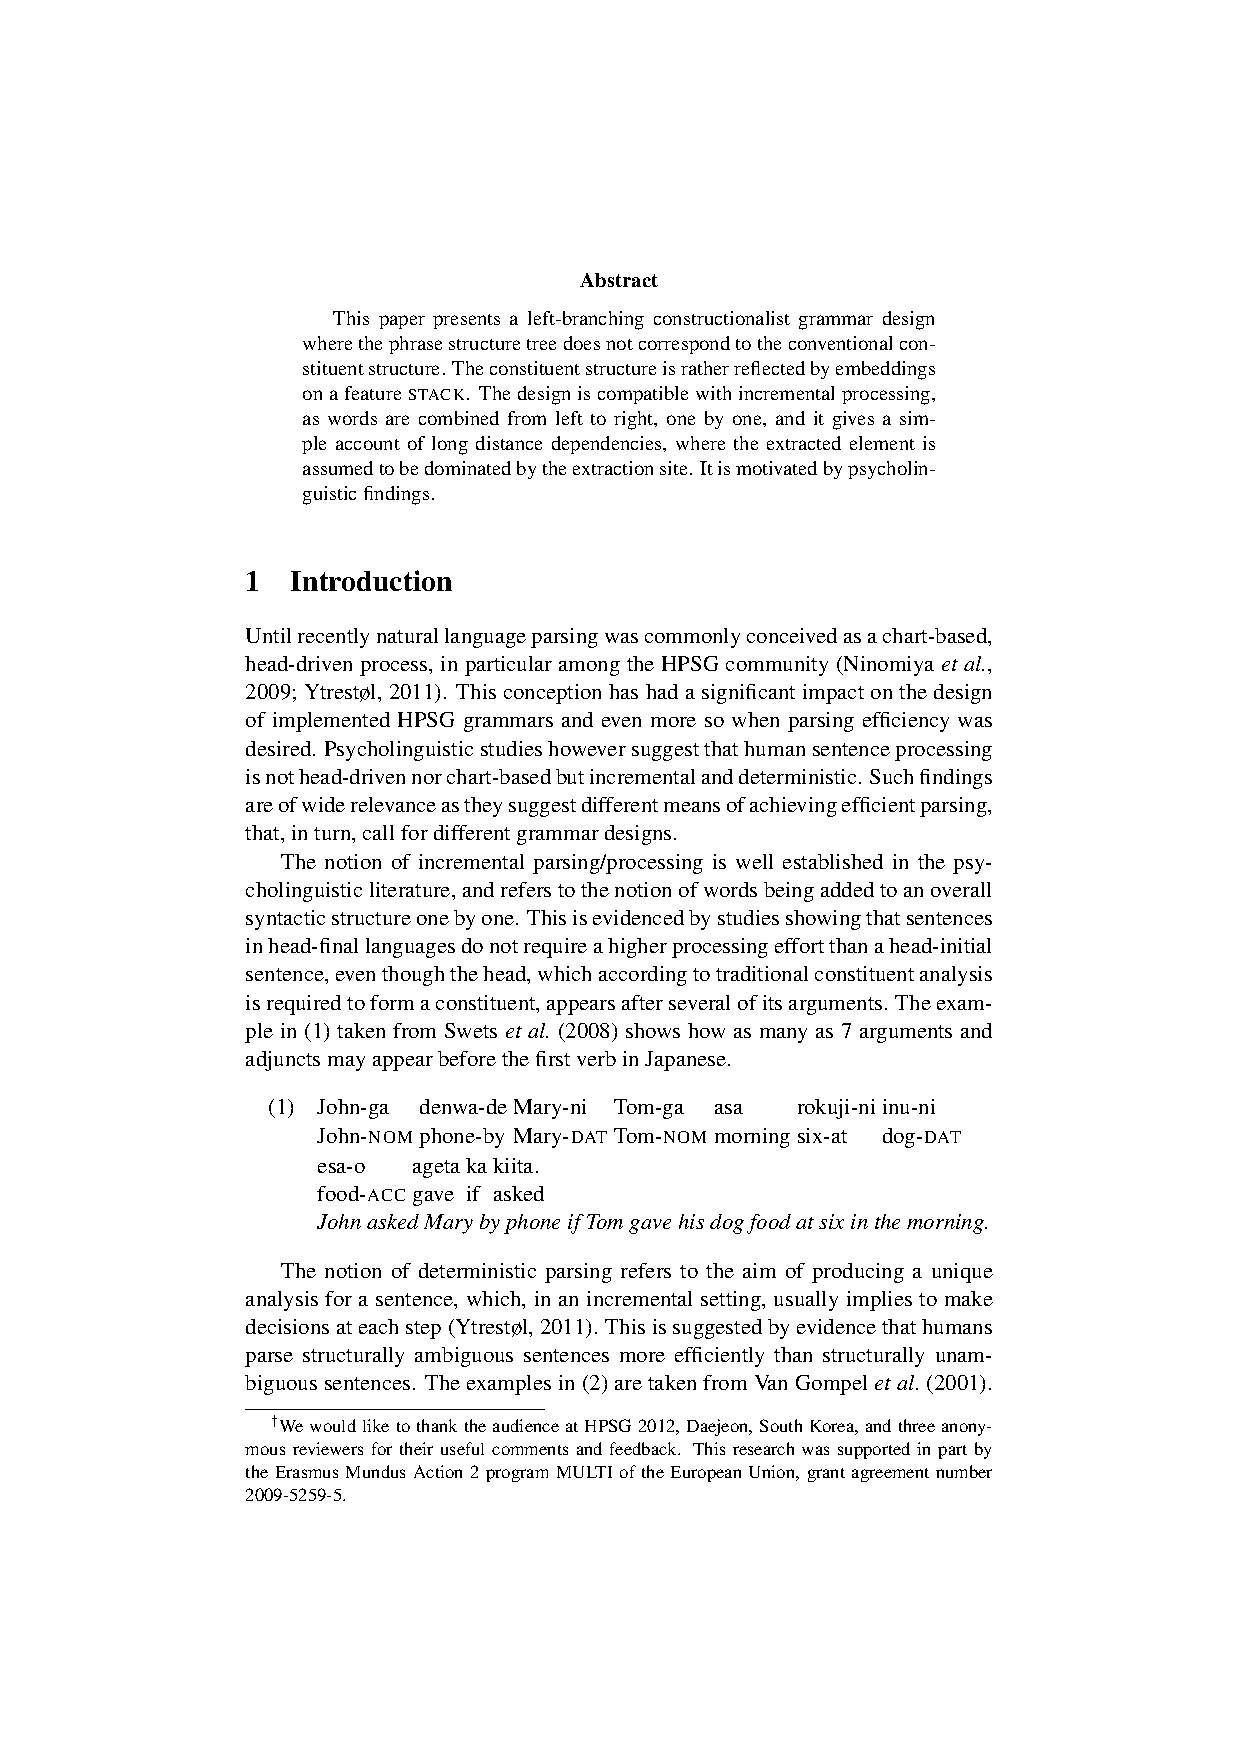
\includepdf[pages=-,pagecommand=\thispagestyle{plain}]{Includes/haugereid-morey.pdf}
        \setcounter{page}{195}
        \phantomsection
        \addcontentsline{toc}{section}{Emil Ionescu: A Hybrid Type of Ellipsis in Romanian}
\thispagestyle{empty}

\begin{center}
  {\huge\bfseries A Hybrid Type of Ellipsis in Romanian\par}

  \bigskip

~\\
\begingroup
\setlength{\leftskip}{0pt plus 1fill}
\setlength{\rightskip}{0pt plus 1fill}
\setlength{\parindent}{0pt}
\setlength{\parfillskip}{0pt}
  \formatauthor{Emil Ionescu}{\begin{tabular}{@{}c@{}}University of Bucharest\end{tabular}}

\par\endgroup

  \vspace*{8ex}

  Proceedings of the 19th International Conference on\par Head-Driven Phrase Structure Grammar

  \bigskip

  Chungnam National University Daejeon

  \medskip

  Stefan Müller (Editor)

  \medskip

  2012

  \medskip

  CSLI Publications

  \medskip

  pages 195--215

  \medskip

  \url{http://csli-publications.stanford.edu/HPSG/2012}
\end{center}
\vfill

\noindent



\vfill
\noindent
% APA Style
Ionescu, Emil. 2012. A Hybrid Type of Ellipsis in Romanian. In Müller, Stefan (Ed.), \emph{{Proceedings of the 19th International Conference on Head-Driven Phrase Structure Grammar, Chungnam National University Daejeon}}, 195--215. Stanford,
CA: CSLI Publications. \hfill\href{http://creativecommons.org/licenses/by/4.0/}{\includegraphics[height=.75em]{Includes/ccby.eps}}

\newpage
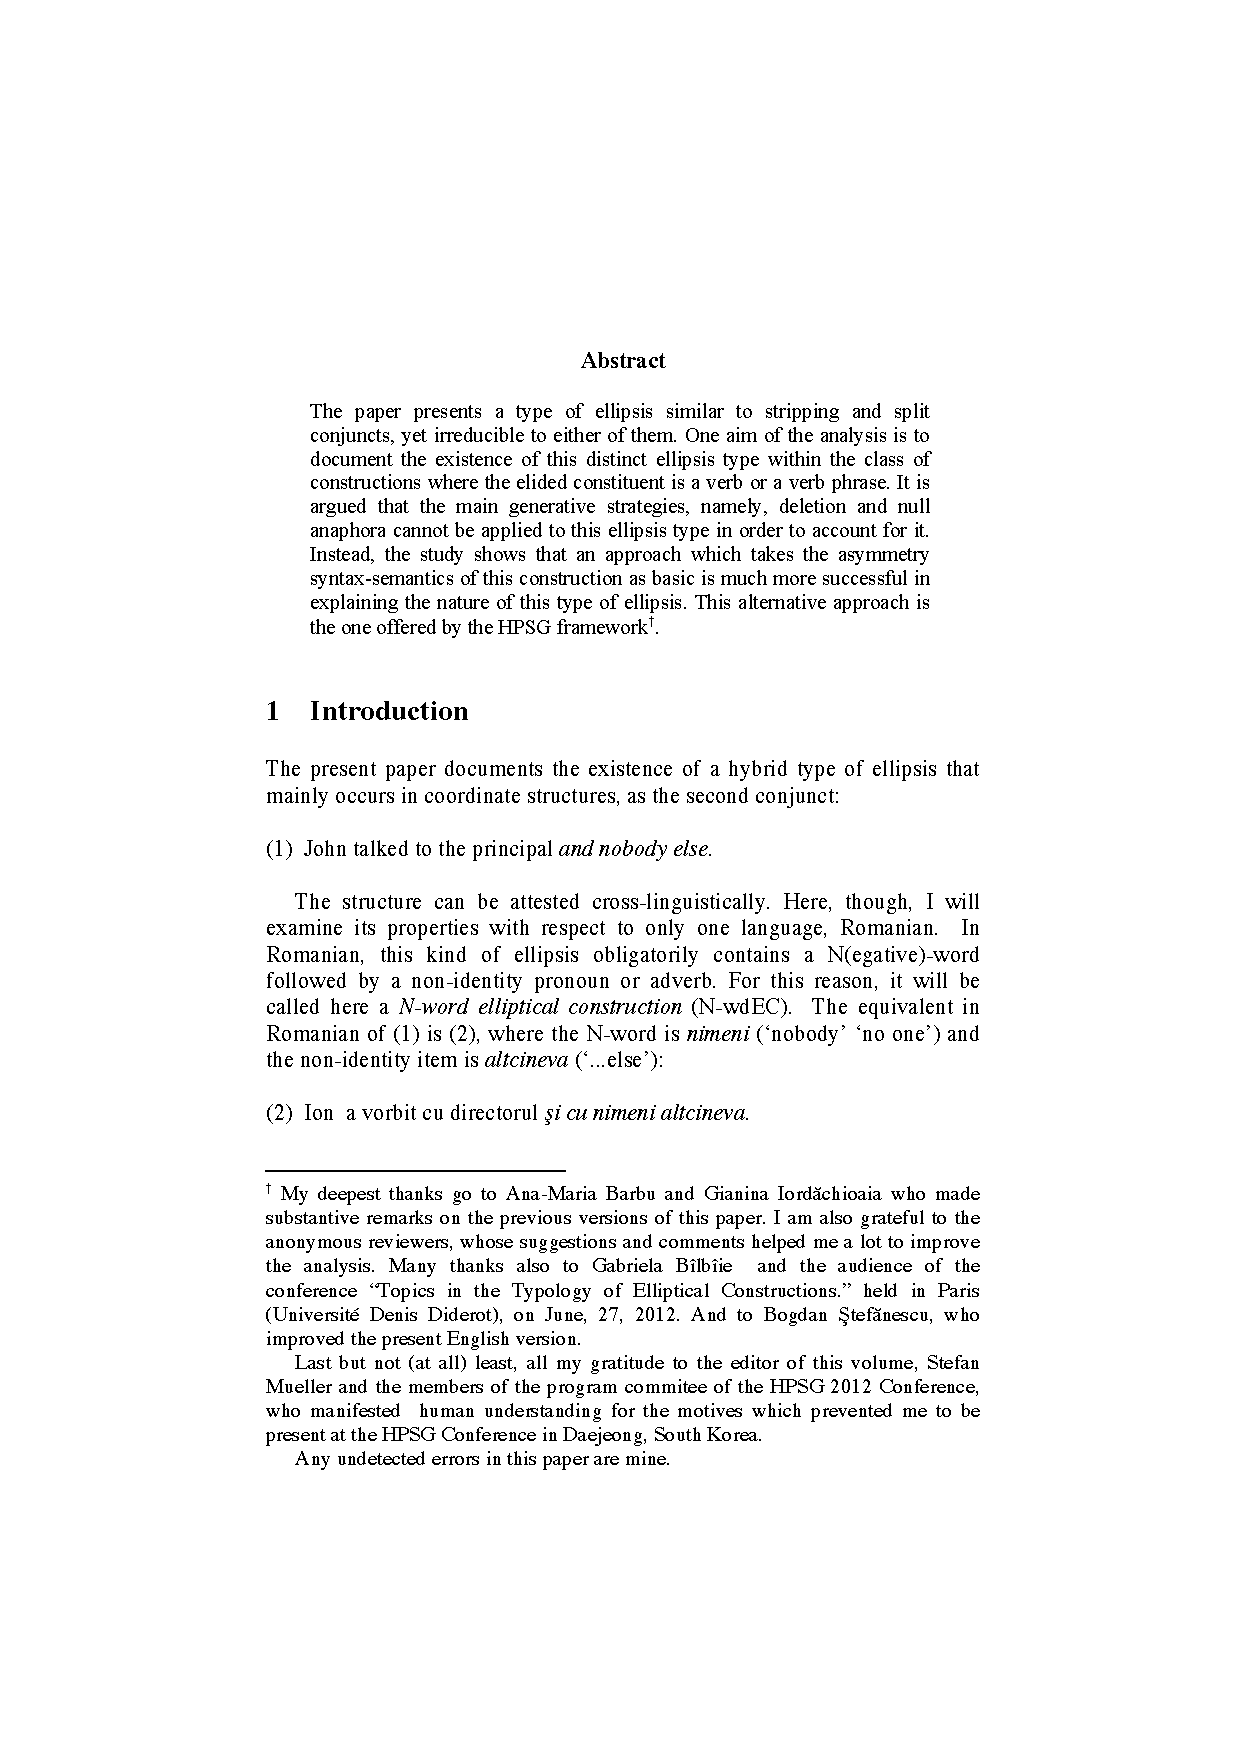
\includepdf[pages=-,pagecommand=\thispagestyle{plain}]{Includes/ionescu.pdf}
        \setcounter{page}{216}
        \phantomsection
        \addcontentsline{toc}{section}{Mija Kim: Syntactic Types of \emph{as}-Parentheticals in Korean}
\thispagestyle{empty}

\begin{center}
  {\huge\bfseries Syntactic Types of \emph{as}-Parentheticals in Korean\par}

  \bigskip

~\\
\begingroup
\setlength{\leftskip}{0pt plus 1fill}
\setlength{\rightskip}{0pt plus 1fill}
\setlength{\parindent}{0pt}
\setlength{\parfillskip}{0pt}
  \formatauthor{Mija Kim}{\begin{tabular}{@{}c@{}}Kyung Hee University\end{tabular}}

\par\endgroup

  \vspace*{8ex}

  Proceedings of the 19th International Conference on\par Head-Driven Phrase Structure Grammar

  \bigskip

  Chungnam National University Daejeon

  \medskip

  Stefan Müller (Editor)

  \medskip

  2012

  \medskip

  CSLI Publications

  \medskip

  pages 216--231

  \medskip

  \url{http://csli-publications.stanford.edu/HPSG/2012}
\end{center}
\vfill

\noindent



\vfill
\noindent
% APA Style
Kim, Mija. 2012. Syntactic Types of \emph{as}-Parentheticals in Korean. In Müller, Stefan (Ed.), \emph{{Proceedings of the 19th International Conference on Head-Driven Phrase Structure Grammar, Chungnam National University Daejeon}}, 216--231. Stanford,
CA: CSLI Publications. \hfill\href{http://creativecommons.org/licenses/by/4.0/}{\includegraphics[height=.75em]{Includes/ccby.eps}}

\newpage
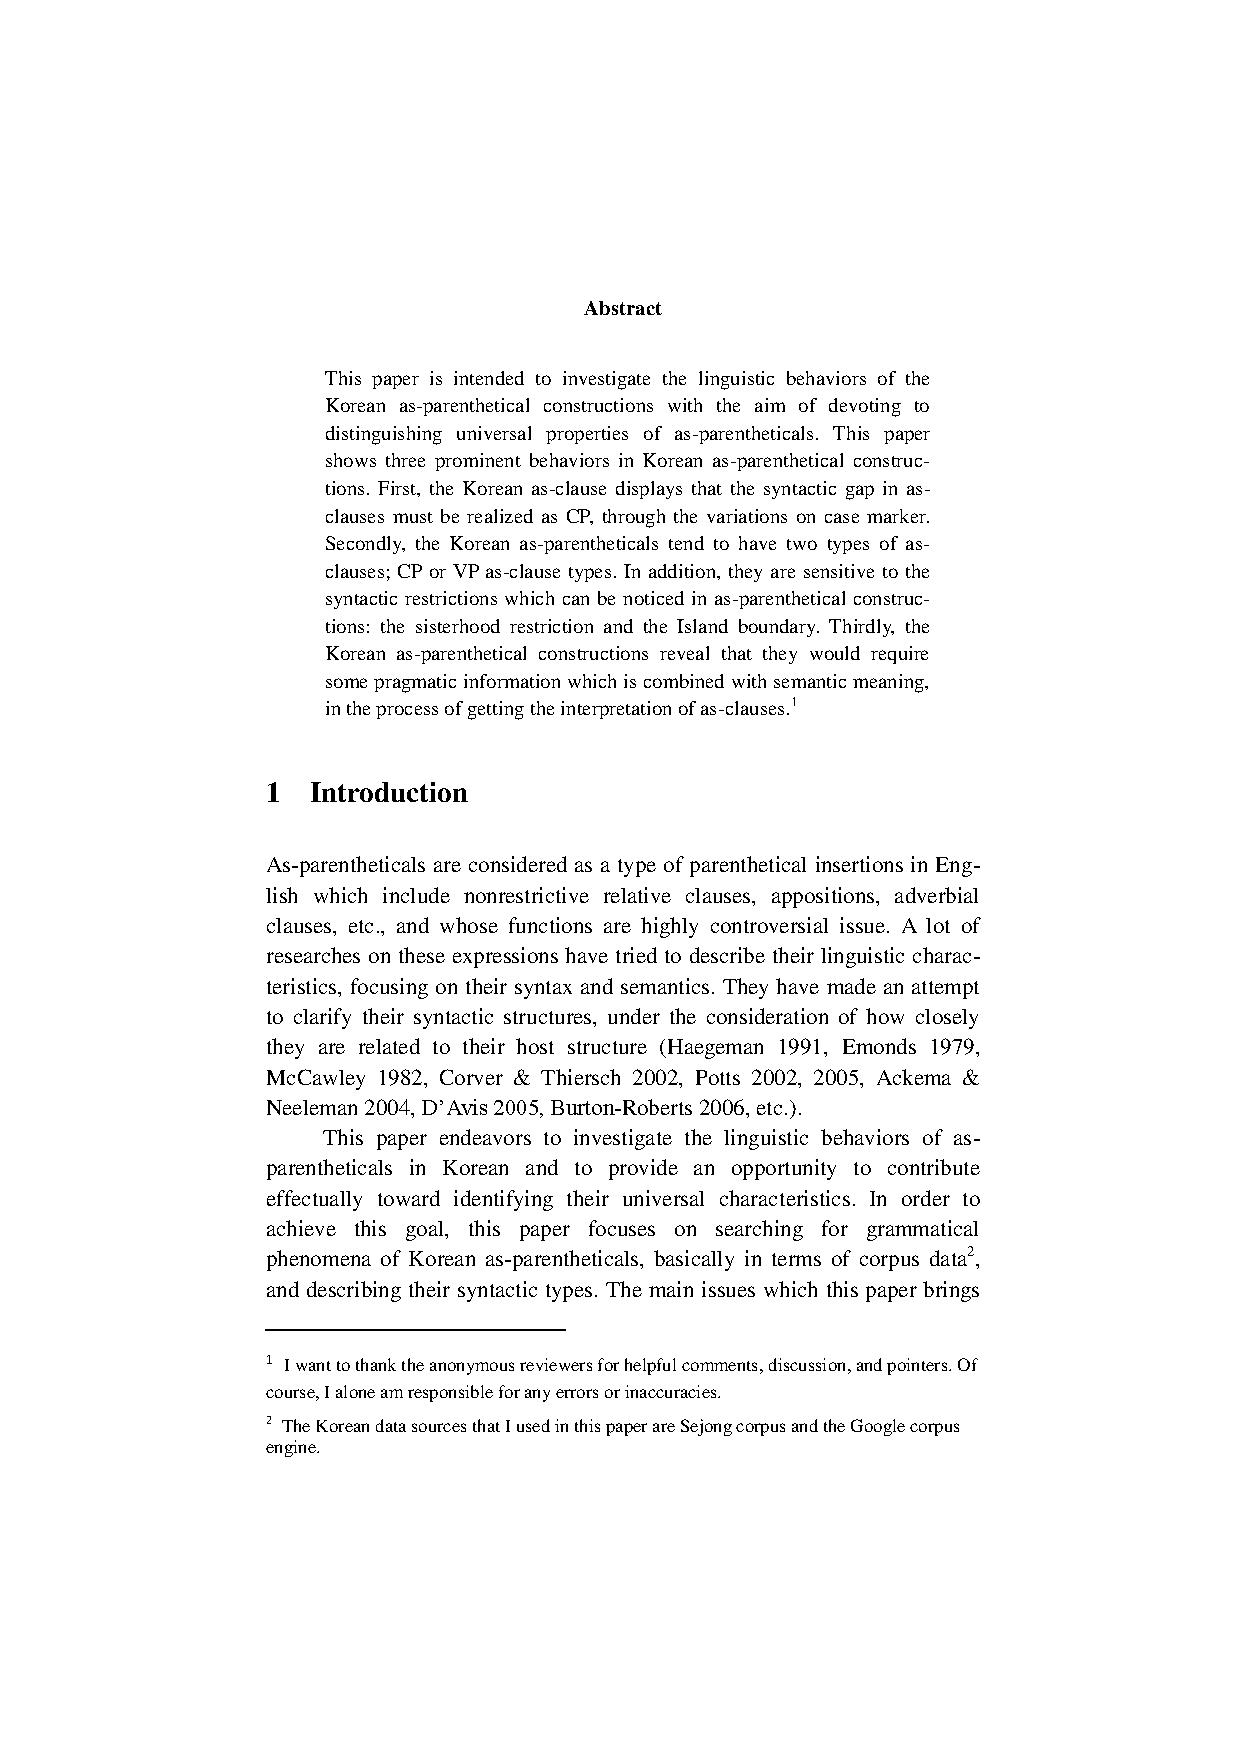
\includepdf[pages=-,pagecommand=\thispagestyle{plain}]{Includes/kim.pdf}
        \setcounter{page}{232}
        \phantomsection
        \addcontentsline{toc}{section}{Hiroki Koga: Past Affix' Selection of Verbal Stems}
\thispagestyle{empty}

\begin{center}
  {\huge\bfseries Past Affix' Selection of Verbal Stems\par}

  \bigskip

~\\
\begingroup
\setlength{\leftskip}{0pt plus 1fill}
\setlength{\rightskip}{0pt plus 1fill}
\setlength{\parindent}{0pt}
\setlength{\parfillskip}{0pt}
  \formatauthor{Hiroki Koga}{\begin{tabular}{@{}c@{}}Saga University\end{tabular}}

\par\endgroup

  \vspace*{8ex}

  Proceedings of the 19th International Conference on\par Head-Driven Phrase Structure Grammar

  \bigskip

  Chungnam National University Daejeon

  \medskip

  Stefan Müller (Editor)

  \medskip

  2012

  \medskip

  CSLI Publications

  \medskip

  pages 232--250

  \medskip

  \url{http://csli-publications.stanford.edu/HPSG/2012}
\end{center}
\vfill

\noindent



\vfill
\noindent
% APA Style
Koga, Hiroki. 2012. Past Affix' Selection of Verbal Stems. In Müller, Stefan (Ed.), \emph{{Proceedings of the 19th International Conference on Head-Driven Phrase Structure Grammar, Chungnam National University Daejeon}}, 232--250. Stanford,
CA: CSLI Publications. \hfill\href{http://creativecommons.org/licenses/by/4.0/}{\includegraphics[height=.75em]{Includes/ccby.eps}}

\newpage
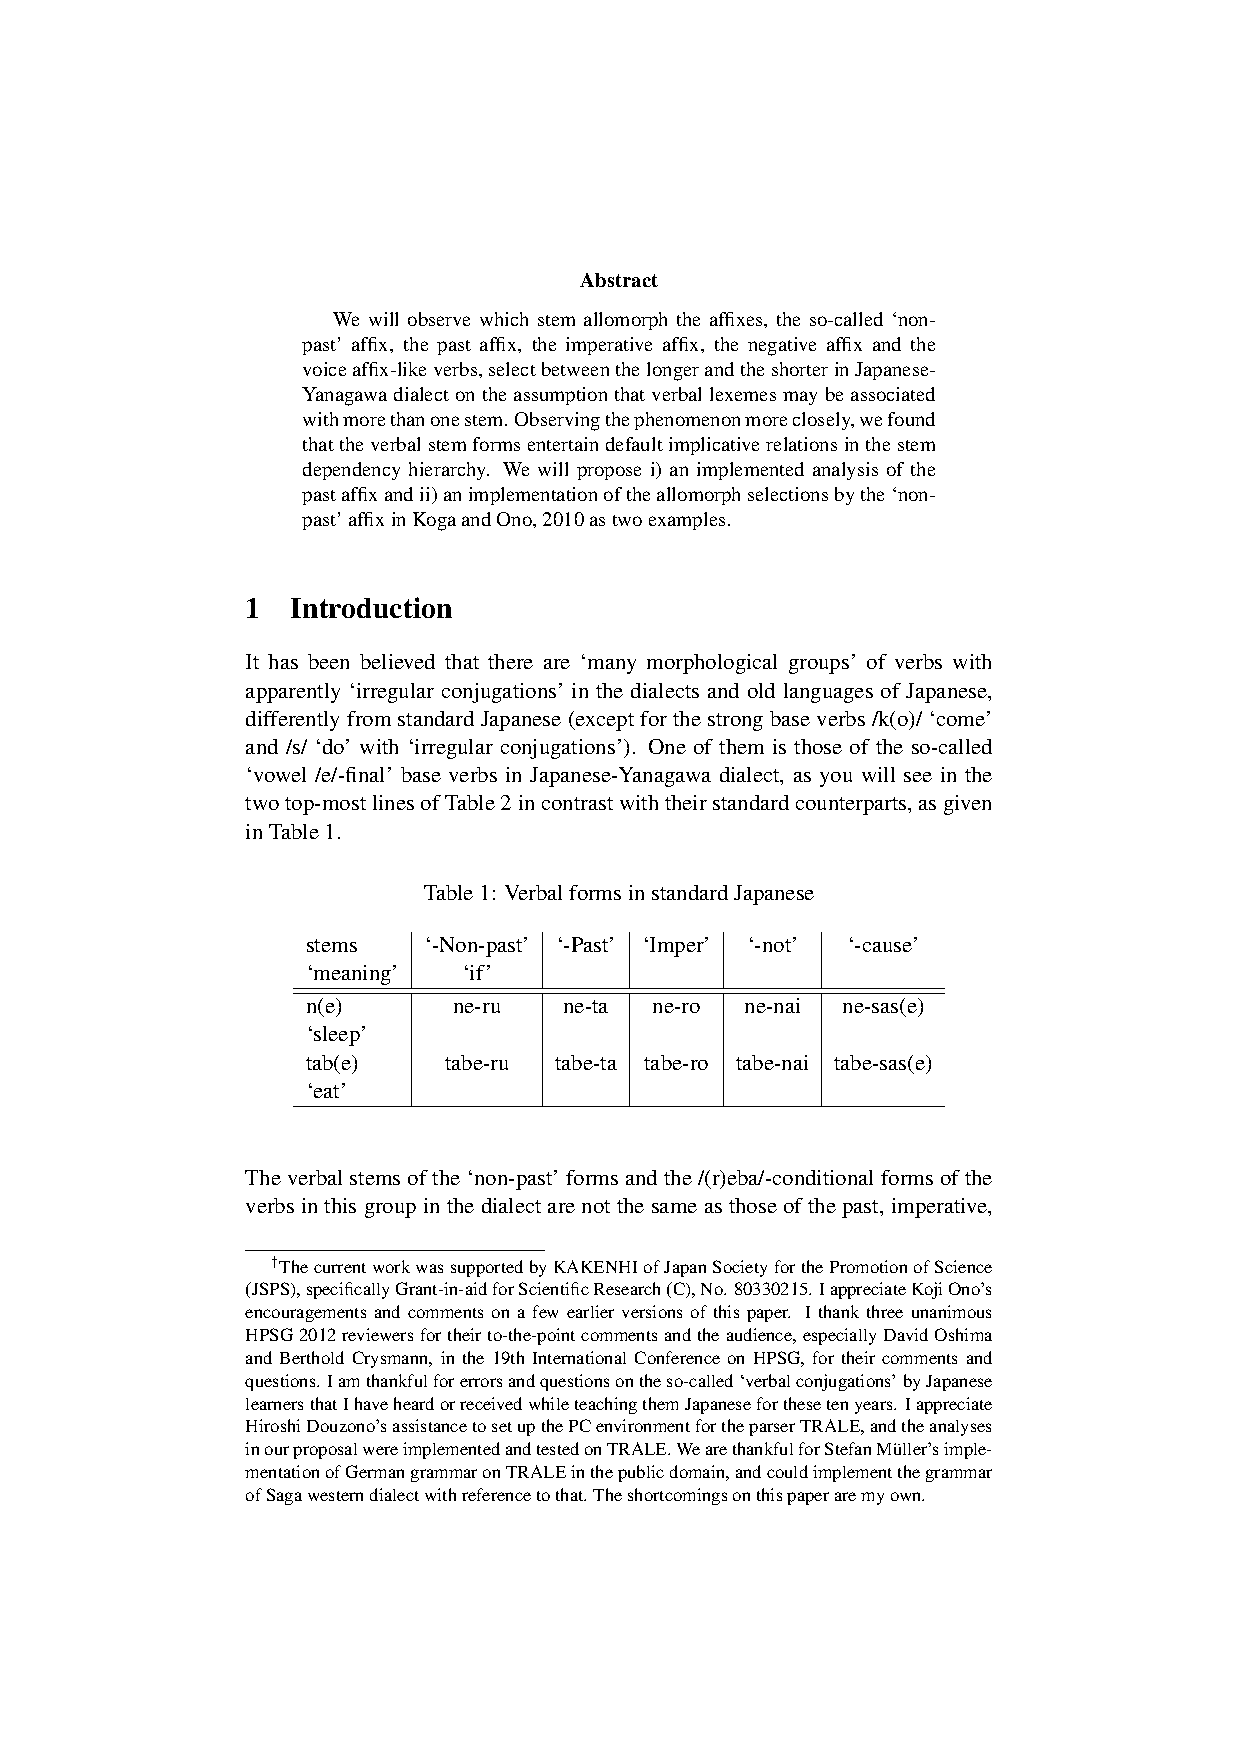
\includepdf[pages=-,pagecommand=\thispagestyle{plain}]{Includes/koga.pdf}
        \setcounter{page}{251}
        \phantomsection
        \addcontentsline{toc}{section}{Juwon Lee: The Direct Evidential \emph{-te} in Korean:\\ Its Interaction with Person and Experiencer Predicates}
\thispagestyle{empty}

\begin{center}
  {\huge\bfseries The Direct Evidential \emph{-te} in Korean:\par Its Interaction with Person and Experiencer Predicates\par}

  \bigskip

~\\
\begingroup
\setlength{\leftskip}{0pt plus 1fill}
\setlength{\rightskip}{0pt plus 1fill}
\setlength{\parindent}{0pt}
\setlength{\parfillskip}{0pt}
  \formatauthor{Juwon Lee}{\begin{tabular}{@{}c@{}}University of Texas at Austin\end{tabular}}

\par\endgroup

  \vspace*{8ex}

  Proceedings of the 19th International Conference on\par Head-Driven Phrase Structure Grammar

  \bigskip

  Chungnam National University Daejeon

  \medskip

  Stefan Müller (Editor)

  \medskip

  2012

  \medskip

  CSLI Publications

  \medskip

  pages 251--271

  \medskip

  \url{http://csli-publications.stanford.edu/HPSG/2012}
\end{center}
\vfill

\noindent



\vfill
\noindent
% APA Style
Lee, Juwon. 2012. The Direct Evidential \emph{-te} in Korean:  Its Interaction with Person and Experiencer Predicates. In Müller, Stefan (Ed.), \emph{{Proceedings of the 19th International Conference on Head-Driven Phrase Structure Grammar, Chungnam National University Daejeon}}, 251--271. Stanford,
CA: CSLI Publications. \hfill\href{http://creativecommons.org/licenses/by/4.0/}{\includegraphics[height=.75em]{Includes/ccby.eps}}

\newpage
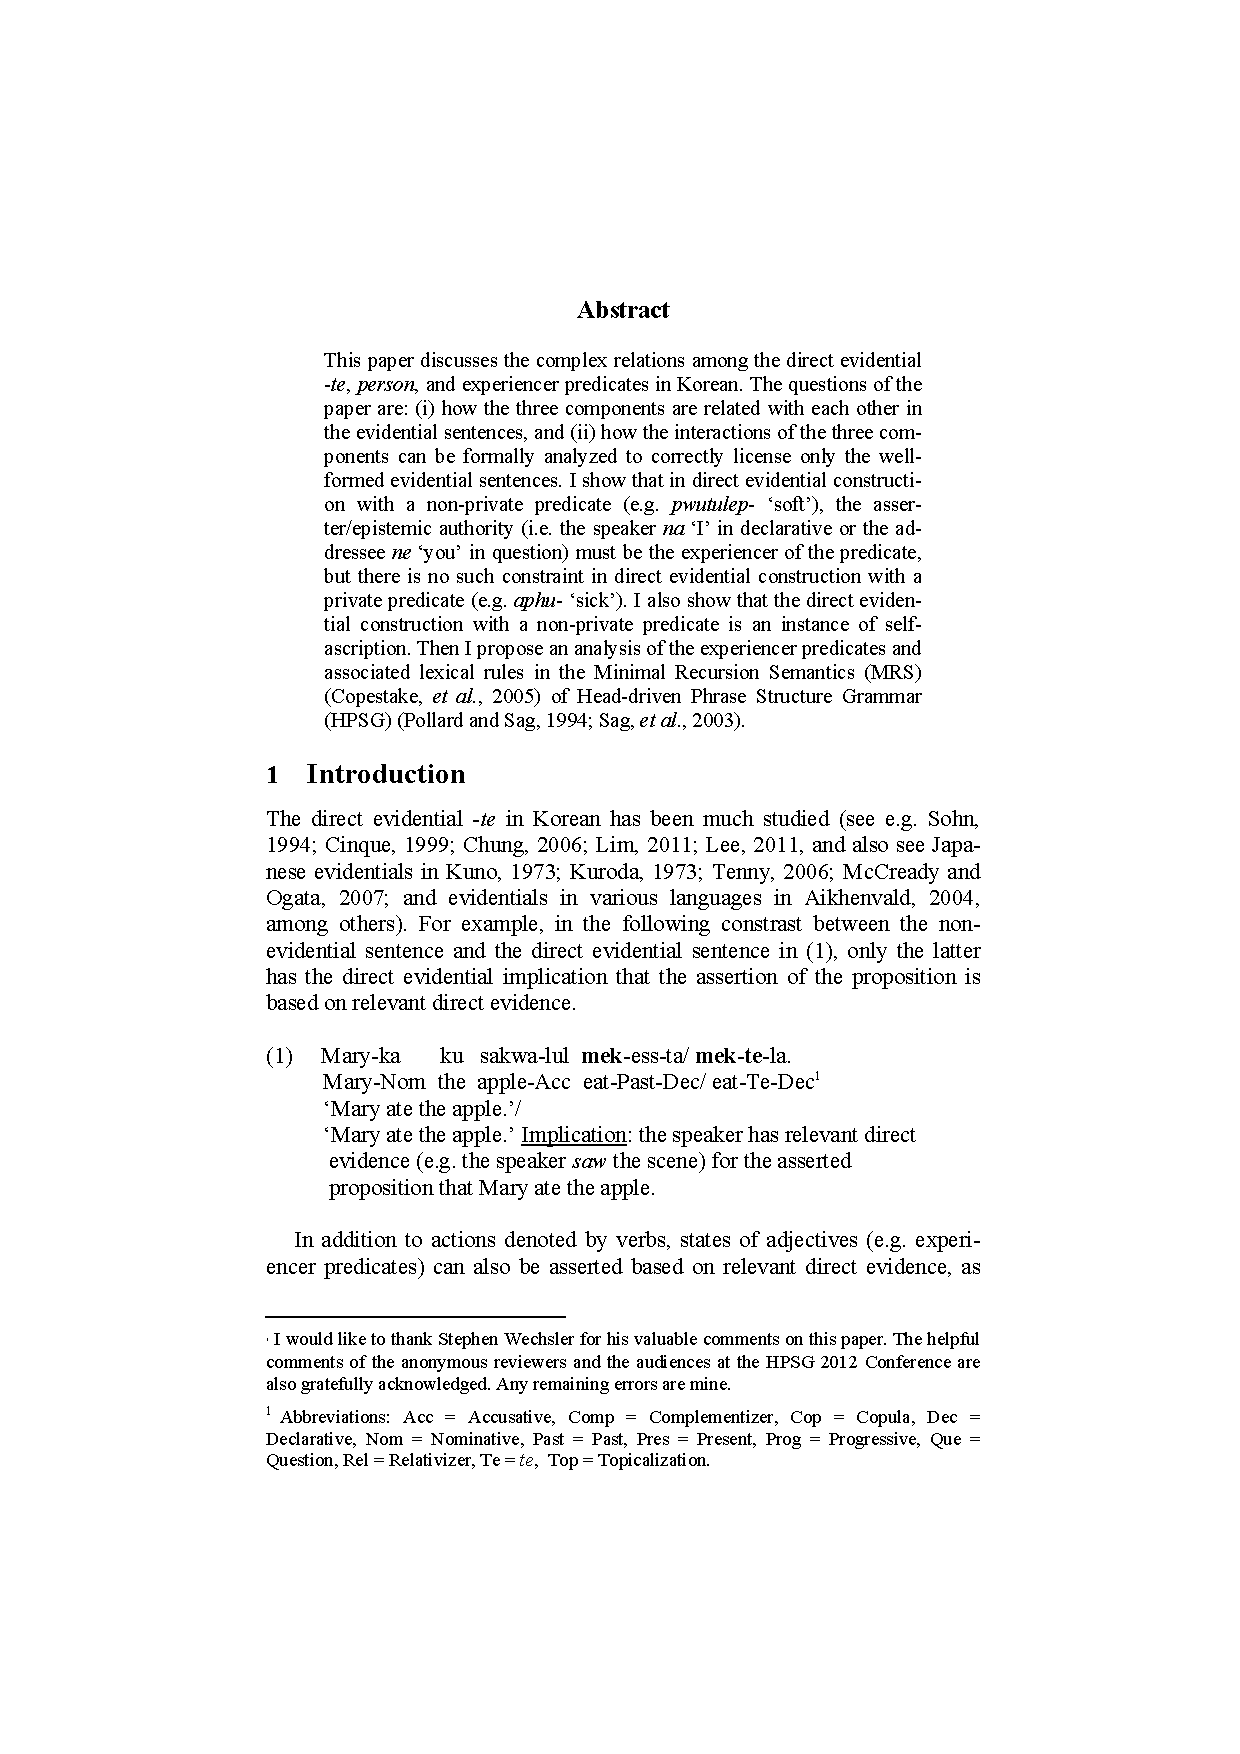
\includepdf[pages=-,pagecommand=\thispagestyle{plain}]{Includes/lee.pdf}
        \setcounter{page}{272}
        \phantomsection
        \addcontentsline{toc}{section}{Yong-hun Lee: A Unified Approach to VP-ellipsis and VP-anaphora}
\thispagestyle{empty}

\begin{center}
  {\huge\bfseries A Unified Approach to VP-ellipsis and VP-anaphora\par}

  \bigskip

~\\
\begingroup
\setlength{\leftskip}{0pt plus 1fill}
\setlength{\rightskip}{0pt plus 1fill}
\setlength{\parindent}{0pt}
\setlength{\parfillskip}{0pt}
  \formatauthor{Yong-hun Lee}{\begin{tabular}{@{}c@{}}Chungnam National University\end{tabular}}

\par\endgroup

  \vspace*{8ex}

  Proceedings of the 19th International Conference on\par Head-Driven Phrase Structure Grammar

  \bigskip

  Chungnam National University Daejeon

  \medskip

  Stefan Müller (Editor)

  \medskip

  2012

  \medskip

  CSLI Publications

  \medskip

  pages 272--291

  \medskip

  \url{http://csli-publications.stanford.edu/HPSG/2012}
\end{center}
\vfill

\noindent



\vfill
\noindent
% APA Style
Lee, Yong-hun. 2012. A Unified Approach to VP-ellipsis and VP-anaphora. In Müller, Stefan (Ed.), \emph{{Proceedings of the 19th International Conference on Head-Driven Phrase Structure Grammar, Chungnam National University Daejeon}}, 272--291. Stanford,
CA: CSLI Publications. \hfill\href{http://creativecommons.org/licenses/by/4.0/}{\includegraphics[height=.75em]{Includes/ccby.eps}}

\newpage
\includepdf[pages=-,pagecommand=\thispagestyle{plain}]{Includes/lee-yong-hun.pdf}
        \setcounter{page}{292}
        \phantomsection
        \addcontentsline{toc}{section}{David Y. Oshima: On the Semantics of the Japanese Infinitive/Gerund-Clause Constructions: Polysemy and Temporal Constraints}
\thispagestyle{empty}

\begin{center}
  {\huge\bfseries On the Semantics of the Japanese Infinitive/Gerund-Clause Constructions: Polysemy and Temporal Constraints\par}

  \bigskip

~\\
\begingroup
\setlength{\leftskip}{0pt plus 1fill}
\setlength{\rightskip}{0pt plus 1fill}
\setlength{\parindent}{0pt}
\setlength{\parfillskip}{0pt}
  \formatauthor{David Y. Oshima}{\begin{tabular}{@{}c@{}}Nagoya University\end{tabular}}

\par\endgroup

  \vspace*{8ex}

  Proceedings of the 19th International Conference on\par Head-Driven Phrase Structure Grammar

  \bigskip

  Chungnam National University Daejeon

  \medskip

  Stefan Müller (Editor)

  \medskip

  2012

  \medskip

  CSLI Publications

  \medskip

  pages 292--309

  \medskip

  \url{http://csli-publications.stanford.edu/HPSG/2012}
\end{center}
\vfill

\noindent



\vfill
\noindent
% APA Style
Oshima, David Y. 2012. On the Semantics of the Japanese Infinitive/Gerund-Clause Constructions: Polysemy and Temporal Constraints. In Müller, Stefan (Ed.), \emph{{Proceedings of the 19th International Conference on Head-Driven Phrase Structure Grammar, Chungnam National University Daejeon}}, 292--309. Stanford,
CA: CSLI Publications. \hfill\href{http://creativecommons.org/licenses/by/4.0/}{\includegraphics[height=.75em]{Includes/ccby.eps}}

\newpage
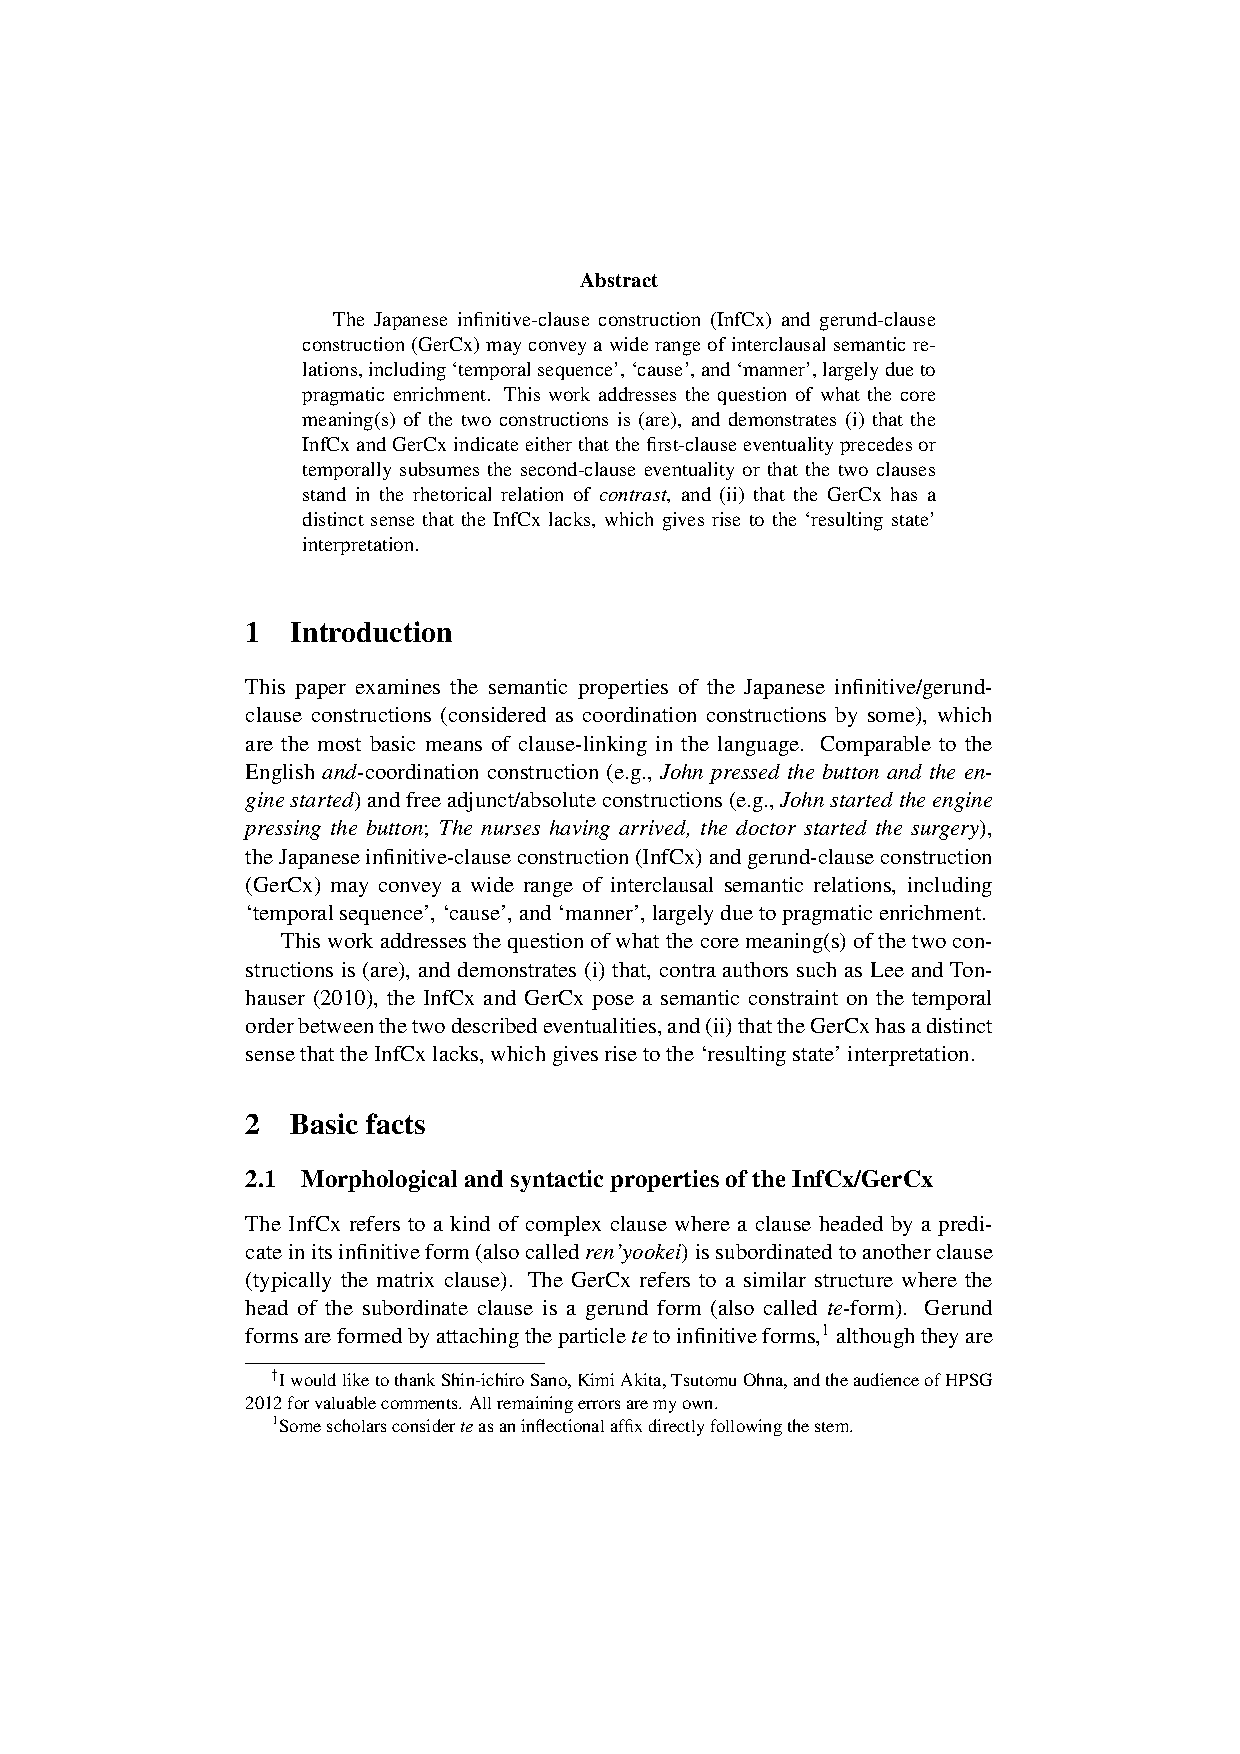
\includepdf[pages=-,pagecommand=\thispagestyle{plain}]{Includes/oshima.pdf}
        \setcounter{page}{310}
        \phantomsection
        \addcontentsline{toc}{section}{Dong-woo Park: An HPSG Approach to English Comparative Inversion}
\thispagestyle{empty}

\begin{center}
  {\huge\bfseries An HPSG Approach to English Comparative Inversion\par}

  \bigskip

~\\
\begingroup
\setlength{\leftskip}{0pt plus 1fill}
\setlength{\rightskip}{0pt plus 1fill}
\setlength{\parindent}{0pt}
\setlength{\parfillskip}{0pt}
  \formatauthor{Dong-woo Park}{\begin{tabular}{@{}c@{}}Seoul National University\end{tabular}}

\par\endgroup

  \vspace*{8ex}

  Proceedings of the 19th International Conference on\par Head-Driven Phrase Structure Grammar

  \bigskip

  Chungnam National University Daejeon

  \medskip

  Stefan Müller (Editor)

  \medskip

  2012

  \medskip

  CSLI Publications

  \medskip

  pages 310--329

  \medskip

  \url{http://csli-publications.stanford.edu/HPSG/2012}
\end{center}
\vfill

\noindent



\vfill
\noindent
% APA Style
Park, Dong-woo. 2012. An HPSG Approach to English Comparative Inversion. In Müller, Stefan (Ed.), \emph{{Proceedings of the 19th International Conference on Head-Driven Phrase Structure Grammar, Chungnam National University Daejeon}}, 310--329. Stanford,
CA: CSLI Publications. \hfill\href{http://creativecommons.org/licenses/by/4.0/}{\includegraphics[height=.75em]{Includes/ccby.eps}}

\newpage
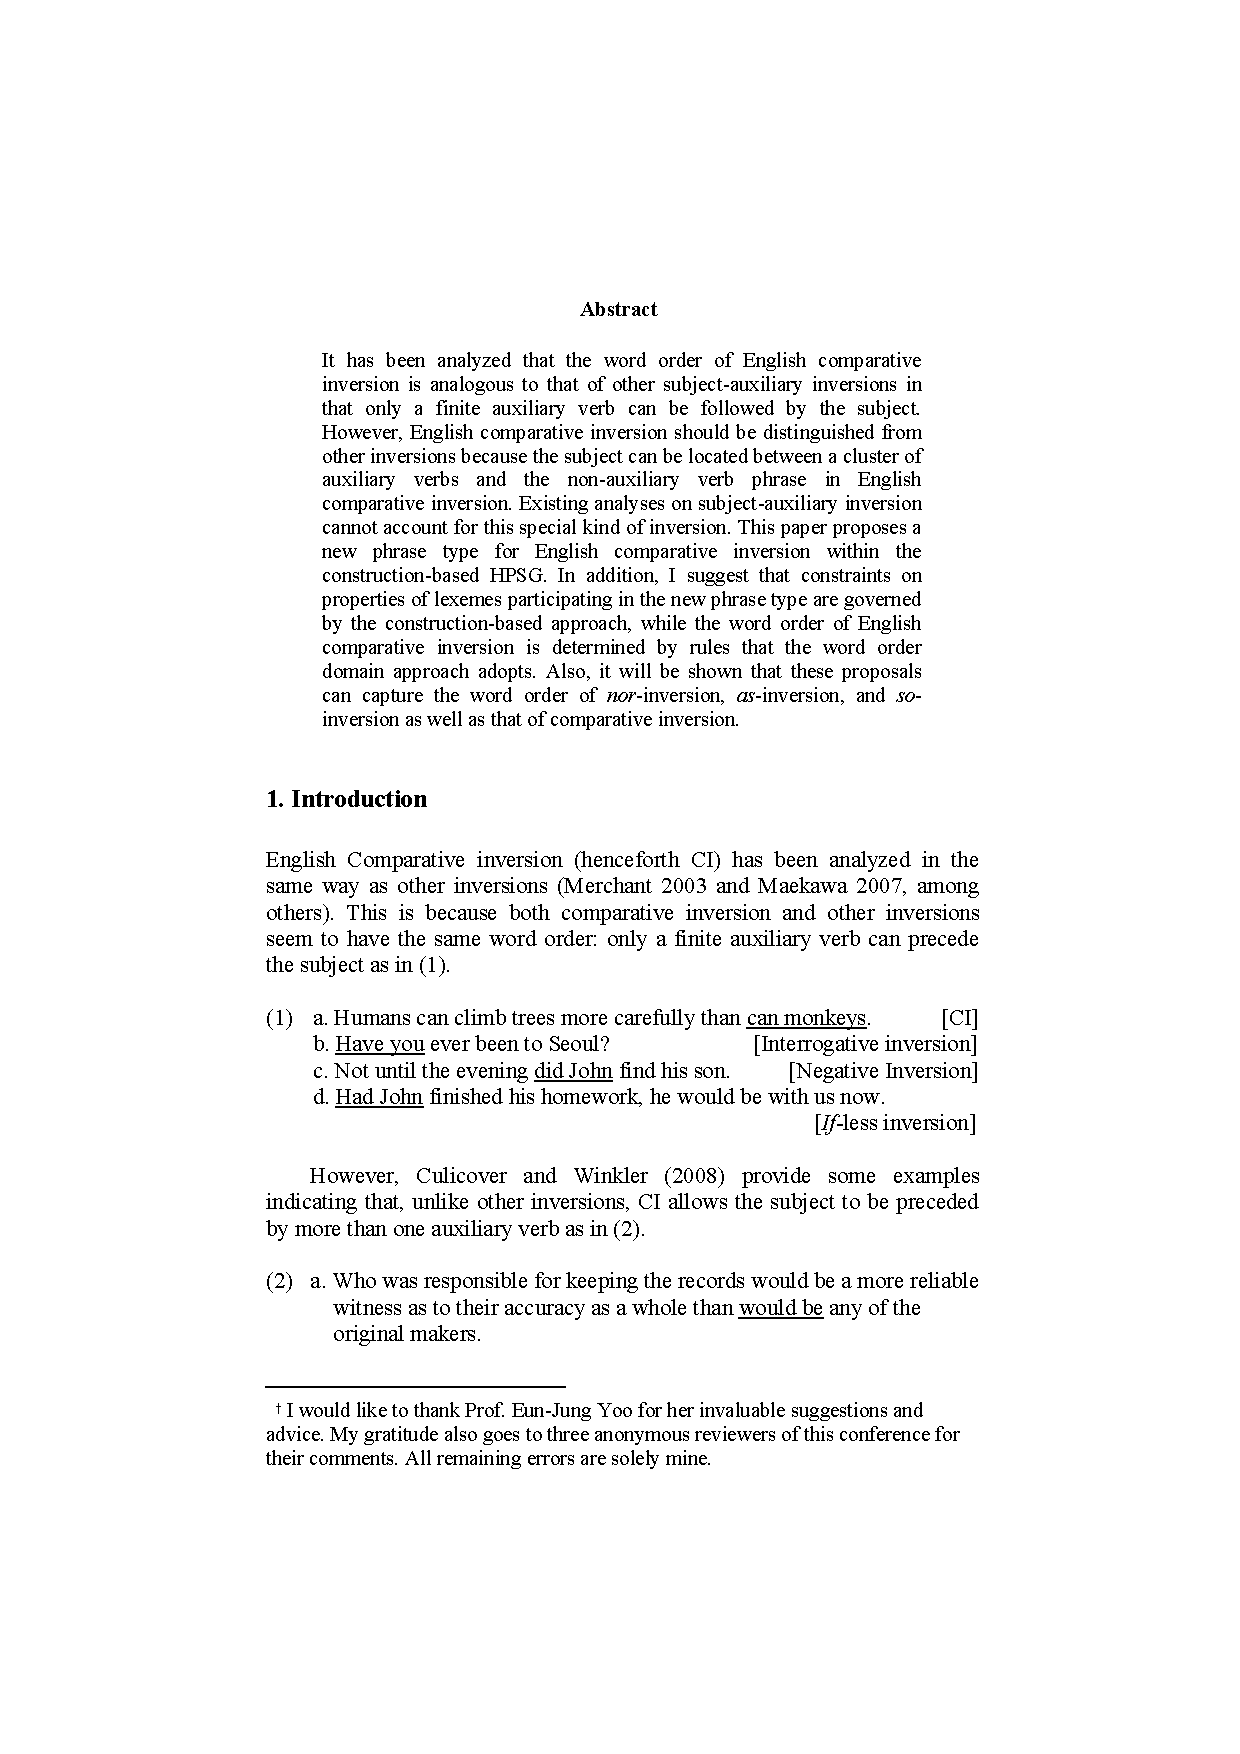
\includepdf[pages=-,pagecommand=\thispagestyle{plain}]{Includes/park.pdf}
        \setcounter{page}{330}
        \phantomsection
        \addcontentsline{toc}{section}{Sanghoun Song, Emily M. Bender: Individual Constraints for Information Structure}
\thispagestyle{empty}

\begin{center}
  {\huge\bfseries Individual Constraints for Information Structure\par}

  \bigskip

~\\
\begingroup
\setlength{\leftskip}{0pt plus 1fill}
\setlength{\rightskip}{0pt plus 1fill}
\setlength{\parindent}{0pt}
\setlength{\parfillskip}{0pt}
  \formatauthor{Sanghoun Song}{\begin{tabular}{@{}c@{}}University of Washington\end{tabular}}
\formatauthor{Emily M. Bender}{\begin{tabular}{@{}c@{}}University of Washington\end{tabular}}

\par\endgroup

  \vspace*{8ex}

  Proceedings of the 19th International Conference on\par Head-Driven Phrase Structure Grammar

  \bigskip

  Chungnam National University Daejeon

  \medskip

  Stefan Müller (Editor)

  \medskip

  2012

  \medskip

  CSLI Publications

  \medskip

  pages 330--348

  \medskip

  \url{http://csli-publications.stanford.edu/HPSG/2012}
\end{center}
\vfill

\noindent



\vfill
\noindent
% APA Style
Song, Sanghoun, \& Bender, Emily M. 2012. Individual Constraints for Information Structure. In Müller, Stefan (Ed.), \emph{{Proceedings of the 19th International Conference on Head-Driven Phrase Structure Grammar, Chungnam National University Daejeon}}, 330--348. Stanford,
CA: CSLI Publications. \hfill\href{http://creativecommons.org/licenses/by/4.0/}{\includegraphics[height=.75em]{Includes/ccby.eps}}

\newpage
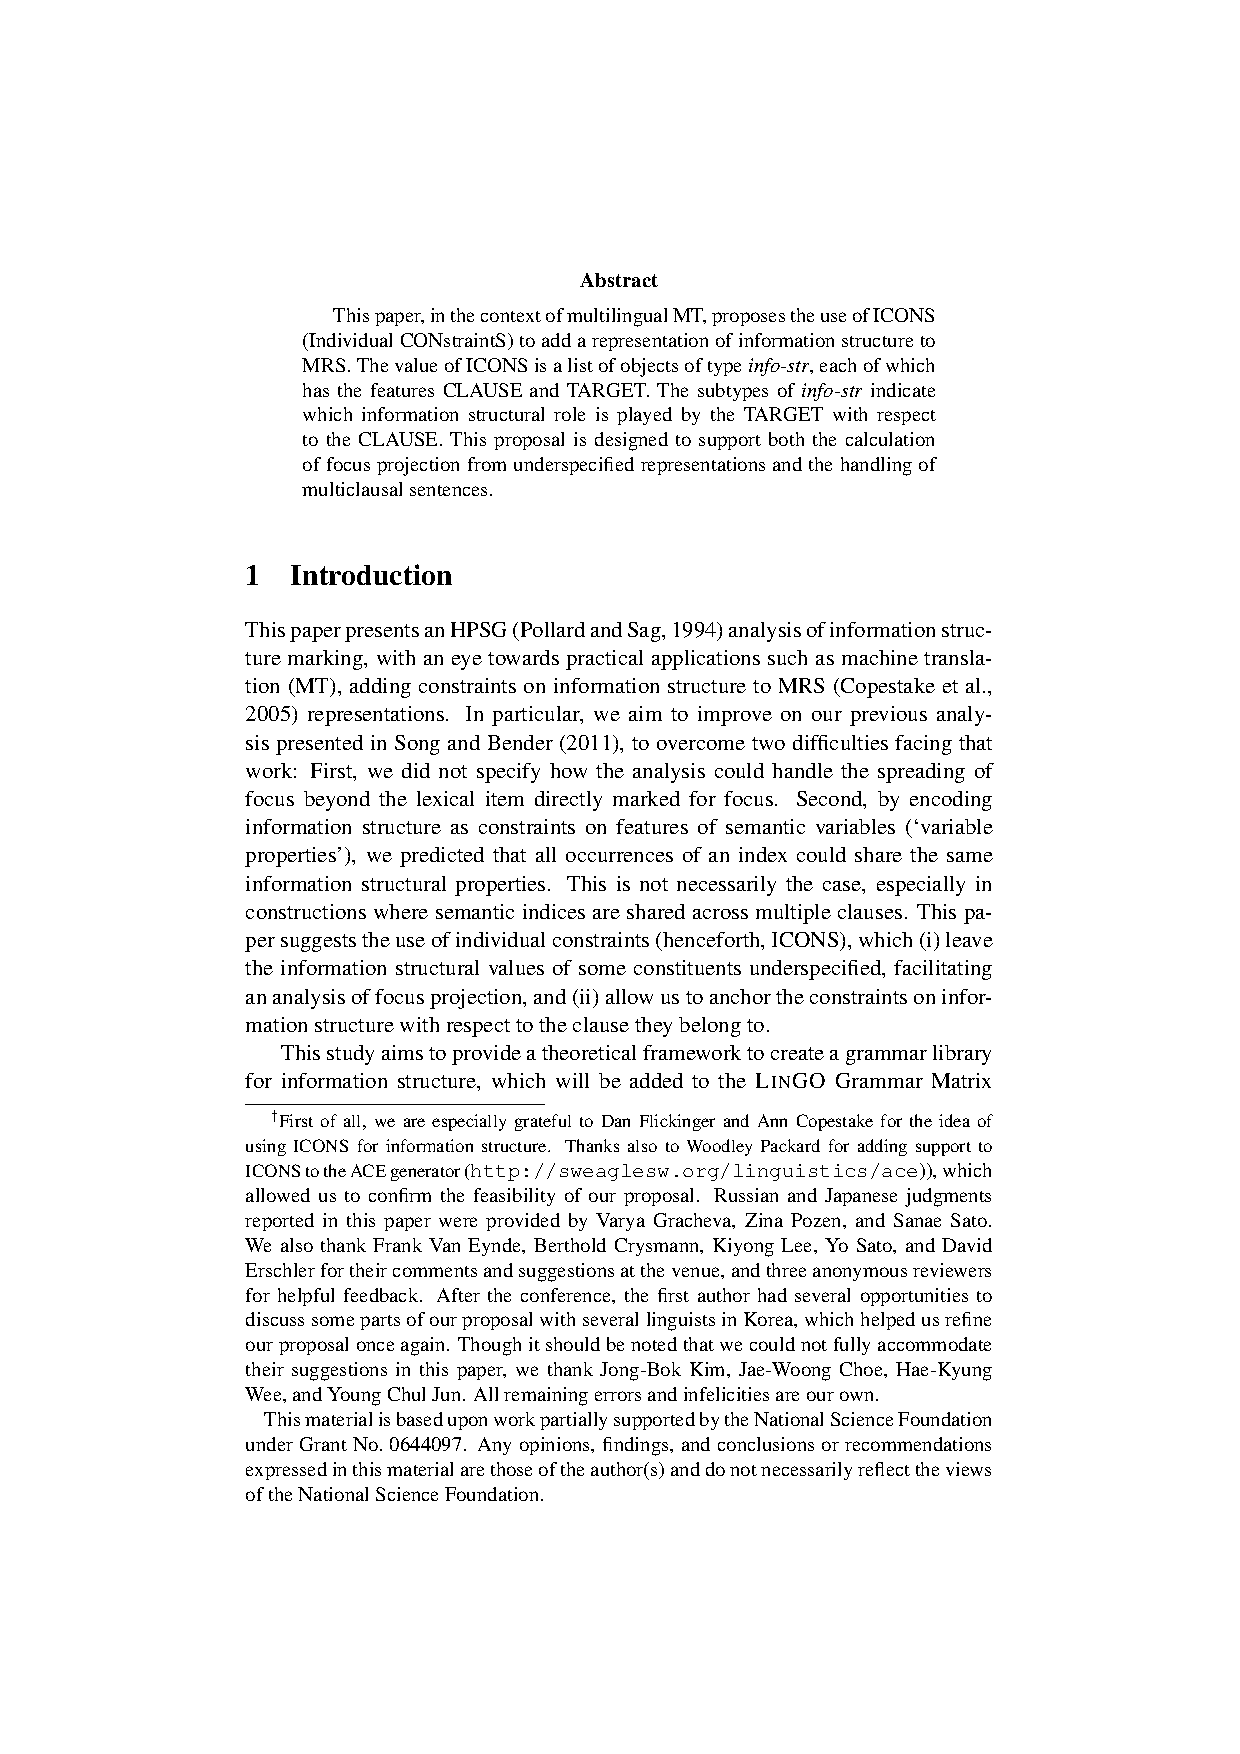
\includepdf[pages=-,pagecommand=\thispagestyle{plain}]{Includes/song-bender.pdf}
        \setcounter{page}{349}
        \phantomsection
        \addcontentsline{toc}{section}{Frank Van Eynde: On the Agreement between Predicative Complements and their Target}
\thispagestyle{empty}

\begin{center}
  {\huge\bfseries On the Agreement between Predicative Complements and their Target\par}

  \bigskip

~\\
\begingroup
\setlength{\leftskip}{0pt plus 1fill}
\setlength{\rightskip}{0pt plus 1fill}
\setlength{\parindent}{0pt}
\setlength{\parfillskip}{0pt}
  \formatauthor{Frank Van Eynde}{\begin{tabular}{@{}c@{}}Centre for Computational Linguistics Department of Linguistics University of Leuven\end{tabular}}

\par\endgroup

  \vspace*{8ex}

  Proceedings of the 19th International Conference on\par Head-Driven Phrase Structure Grammar

  \bigskip

  Chungnam National University Daejeon

  \medskip

  Stefan Müller (Editor)

  \medskip

  2012

  \medskip

  CSLI Publications

  \medskip

  pages 349--367

  \medskip

  \url{http://csli-publications.stanford.edu/HPSG/2012}
\end{center}
\vfill

\noindent



\vfill
\noindent
% APA Style
Van Eynde, Frank. 2012. On the Agreement between Predicative Complements and their Target. In Müller, Stefan (Ed.), \emph{{Proceedings of the 19th International Conference on Head-Driven Phrase Structure Grammar, Chungnam National University Daejeon}}, 349--367. Stanford,
CA: CSLI Publications. \hfill\href{http://creativecommons.org/licenses/by/4.0/}{\includegraphics[height=.75em]{Includes/ccby.eps}}

\newpage
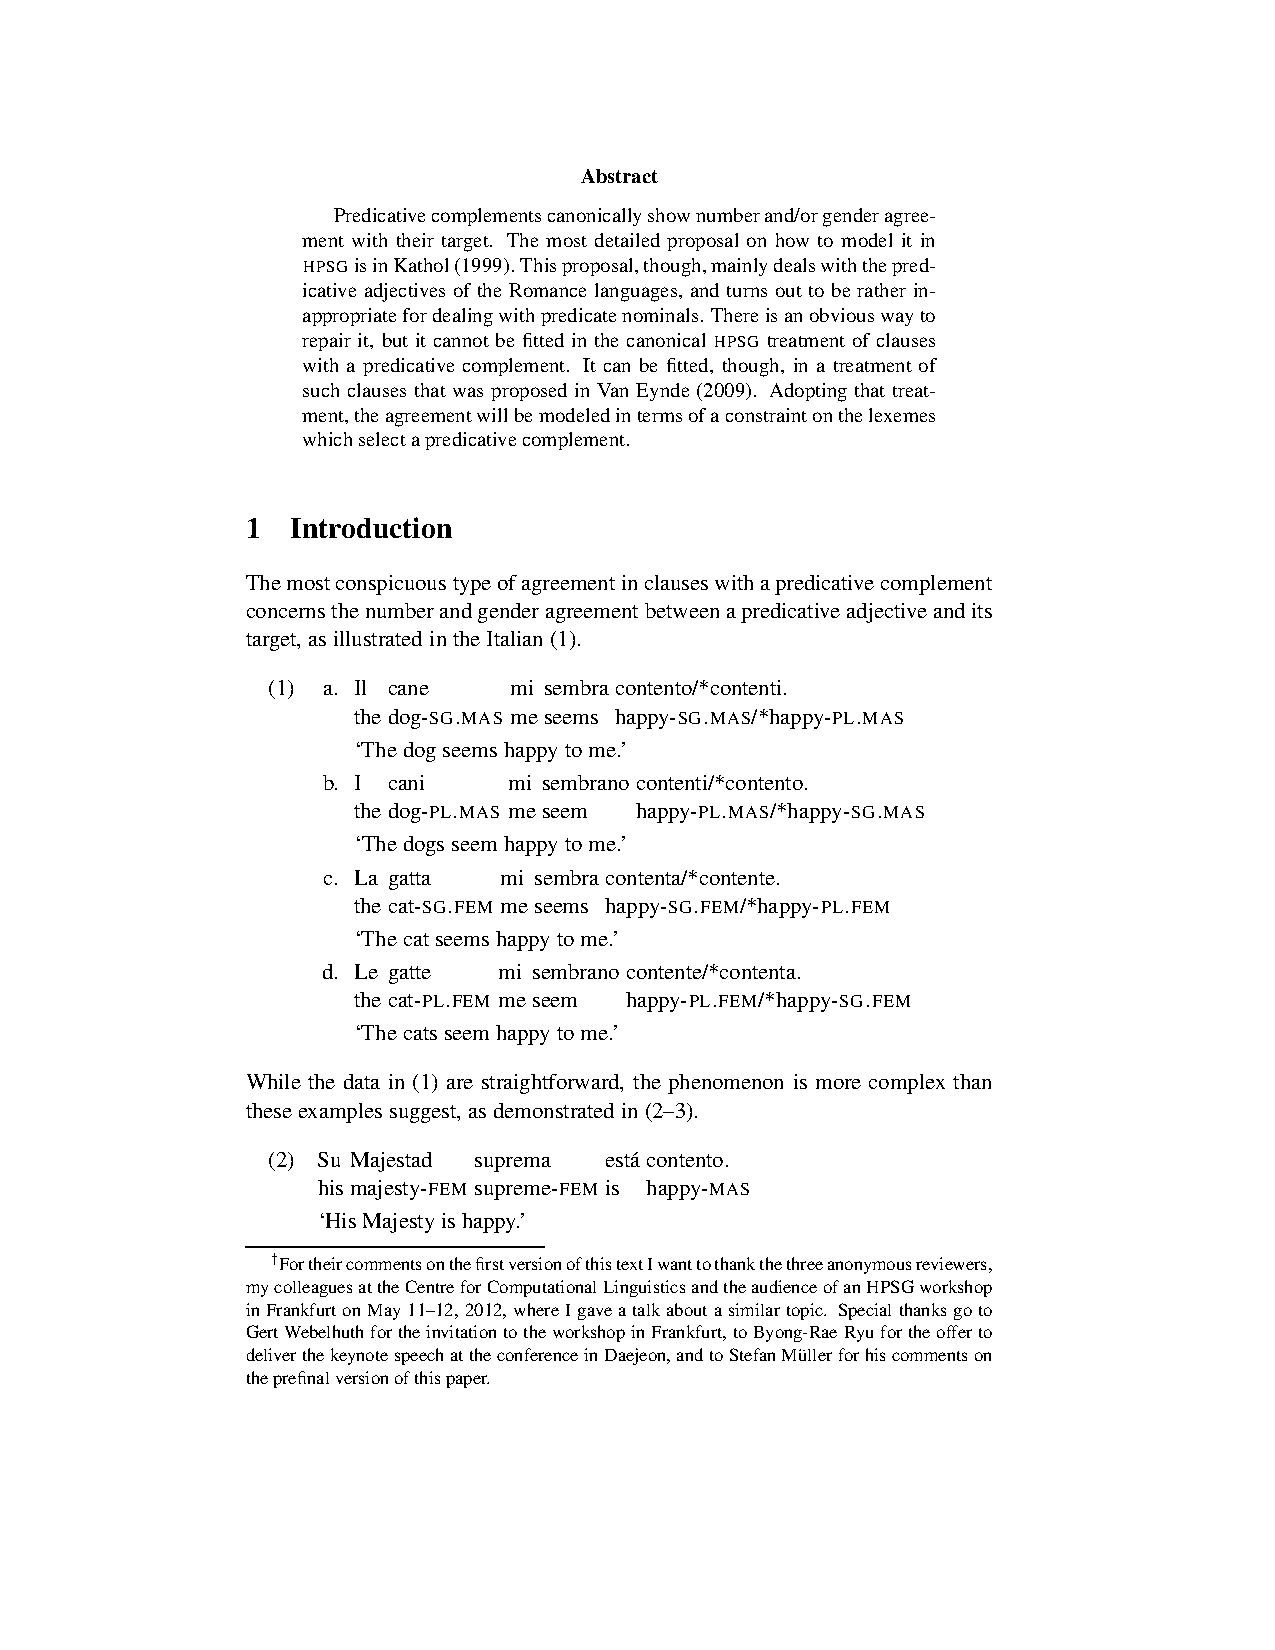
\includepdf[pages=-,pagecommand=\thispagestyle{plain}]{Includes/vaneynde.pdf}
\part{Contributions to the Workshop}
\thispagestyle{empty}
\newpage
        \setcounter{page}{369}
        \phantomsection
        \addcontentsline{toc}{section}{Hee-Don Ahn, Sungeun Cho: Fragments vs. Null Arguments in Korean}
\thispagestyle{empty}

\begin{center}
  {\huge\bfseries Fragments vs. Null Arguments in Korean\par}

  \bigskip

~\\
\begingroup
\setlength{\leftskip}{0pt plus 1fill}
\setlength{\rightskip}{0pt plus 1fill}
\setlength{\parindent}{0pt}
\setlength{\parfillskip}{0pt}
  \formatauthor{Hee-Don Ahn}{\begin{tabular}{@{}c@{}}Konkuk University\end{tabular}}
\formatauthor{Sungeun Cho}{\begin{tabular}{@{}c@{}}Yeungnam University\end{tabular}}

\par\endgroup

  \vspace*{8ex}

  Proceedings of the 19th International Conference on\par Head-Driven Phrase Structure Grammar

  \bigskip

  Chungnam National University Daejeon

  \medskip

  Stefan Müller (Editor)

  \medskip

  2012

  \medskip

  CSLI Publications

  \medskip

  pages 369--387

  \medskip

  \url{http://csli-publications.stanford.edu/HPSG/2012}
\end{center}
\vfill

\noindent



\vfill
\noindent
% APA Style
Ahn, Hee-Don, \& Cho, Sungeun. 2012. Fragments vs. Null Arguments in Korean. In Müller, Stefan (Ed.), \emph{{Proceedings of the 19th International Conference on Head-Driven Phrase Structure Grammar, Chungnam National University Daejeon}}, 369--387. Stanford,
CA: CSLI Publications. \hfill\href{http://creativecommons.org/licenses/by/4.0/}{\includegraphics[height=.75em]{Includes/ccby.eps}}

\newpage
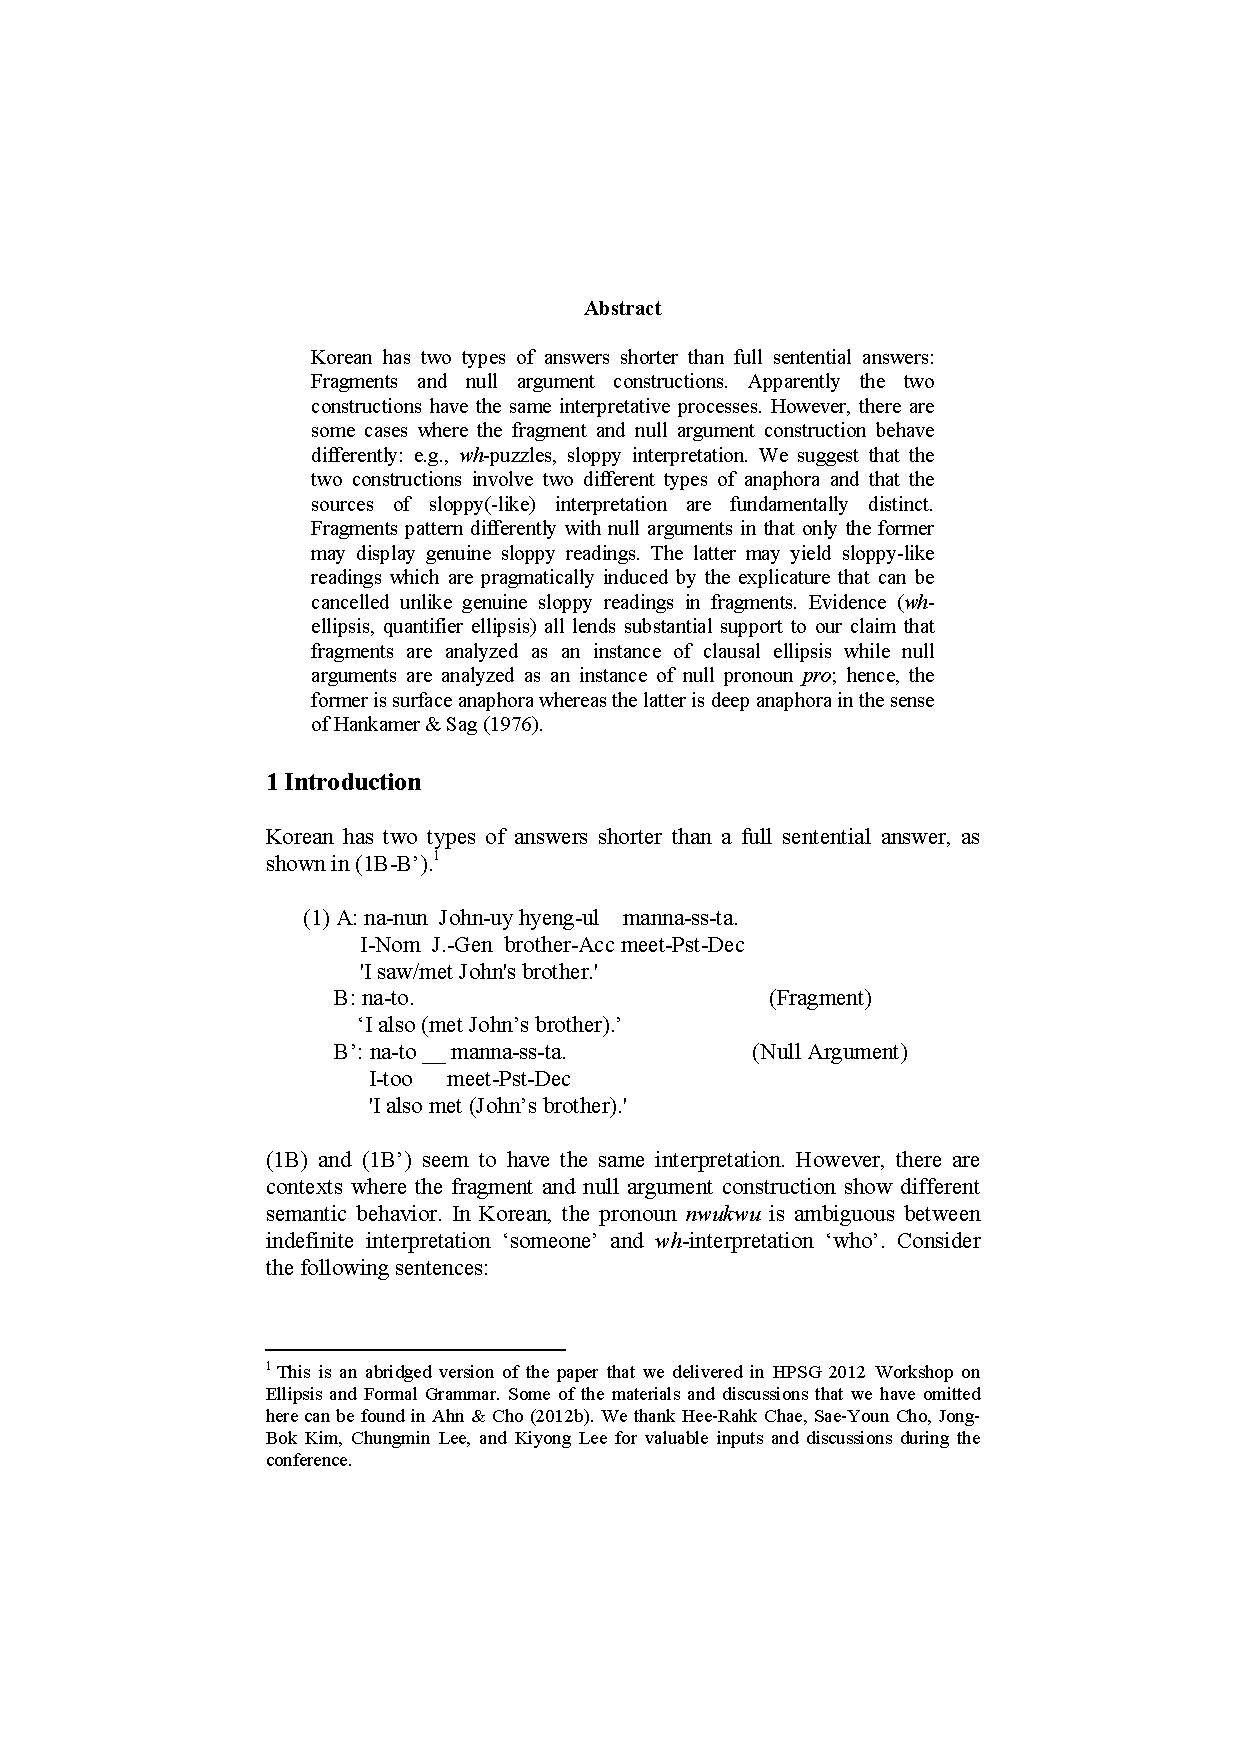
\includepdf[pages=-,pagecommand=\thispagestyle{plain}]{Includes/ahn-cho.pdf}
        \setcounter{page}{388}
        \phantomsection
        \addcontentsline{toc}{section}{Yae-Jee Kim, Sae-Youn Cho: Tense and Honorific Interpretations in Korean Gapping Construction:\\ A Constraint- and Construction-Based Approach}
\thispagestyle{empty}

\begin{center}
  {\huge\bfseries Tense and Honorific Interpretations in Korean Gapping Construction:\par A Constraint- and Construction-Based Approach\par}

  \bigskip

~\\
\begingroup
\setlength{\leftskip}{0pt plus 1fill}
\setlength{\rightskip}{0pt plus 1fill}
\setlength{\parindent}{0pt}
\setlength{\parfillskip}{0pt}
  \formatauthor{Yae-Jee Kim}{\begin{tabular}{@{}c@{}}State University of New York at Buffalo\end{tabular}}
\formatauthor{Sae-Youn Cho}{\begin{tabular}{@{}c@{}}Kangwon National University\end{tabular}}

\par\endgroup

  \vspace*{8ex}

  Proceedings of the 19th International Conference on\par Head-Driven Phrase Structure Grammar

  \bigskip

  Chungnam National University Daejeon

  \medskip

  Stefan Müller (Editor)

  \medskip

  2012

  \medskip

  CSLI Publications

  \medskip

  pages 388--408

  \medskip

  \url{http://csli-publications.stanford.edu/HPSG/2012}
\end{center}
\vfill

\noindent



\vfill
\noindent
% APA Style
Kim, Yae-Jee, \& Cho, Sae-Youn. 2012. Tense and Honorific Interpretations in Korean Gapping Construction:  A Constraint- and Construction-Based Approach. In Müller, Stefan (Ed.), \emph{{Proceedings of the 19th International Conference on Head-Driven Phrase Structure Grammar, Chungnam National University Daejeon}}, 388--408. Stanford,
CA: CSLI Publications. \hfill\href{http://creativecommons.org/licenses/by/4.0/}{\includegraphics[height=.75em]{Includes/ccby.eps}}

\newpage
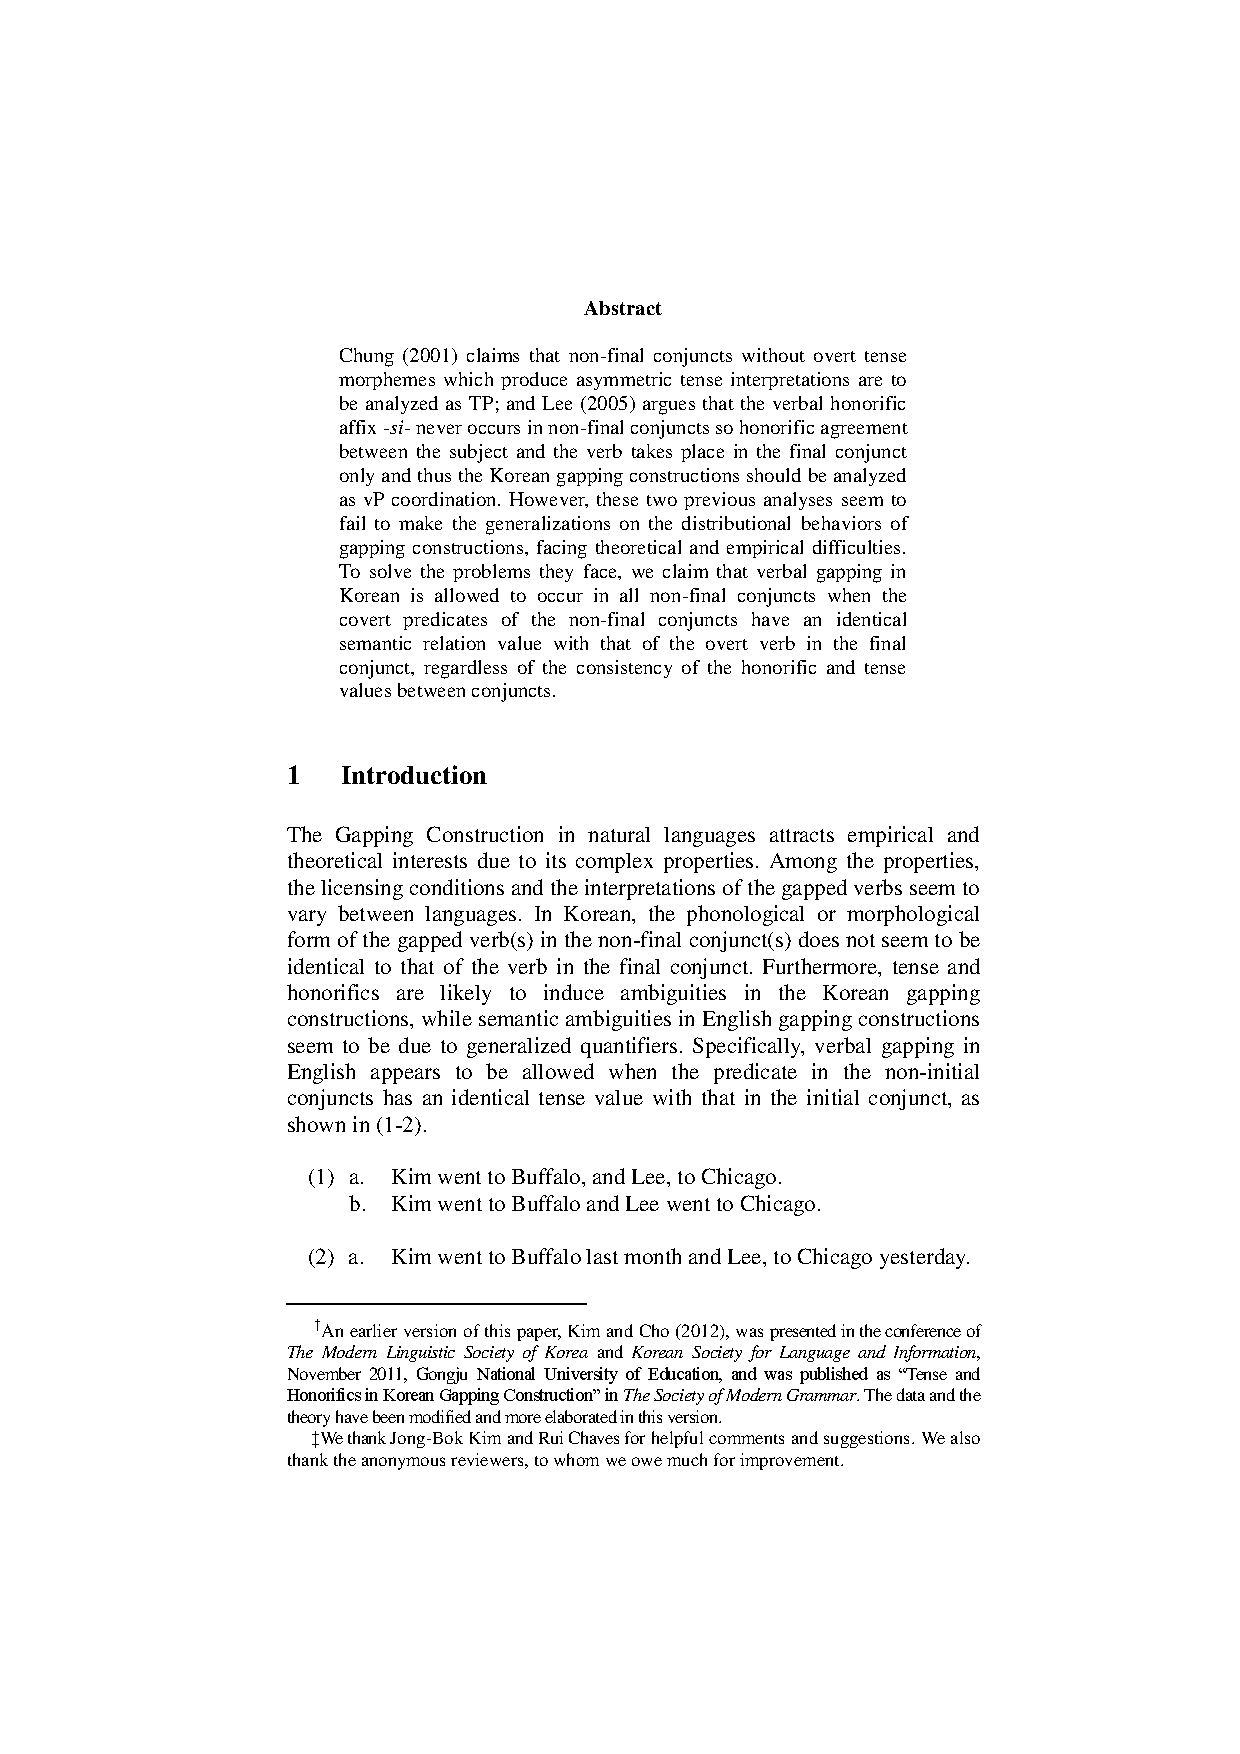
\includepdf[pages=-,pagecommand=\thispagestyle{plain}]{Includes/kim-cho.pdf}
        \setcounter{page}{409}
        \phantomsection
        \addcontentsline{toc}{section}{Gregory M. Kobele: Eliding the Derivation: A Minimalist Formalization of Ellipsis}
\thispagestyle{empty}

\begin{center}
  {\huge\bfseries Eliding the Derivation: A Minimalist Formalization of Ellipsis\par}

  \bigskip

~\\
\begingroup
\setlength{\leftskip}{0pt plus 1fill}
\setlength{\rightskip}{0pt plus 1fill}
\setlength{\parindent}{0pt}
\setlength{\parfillskip}{0pt}
  \formatauthor{Gregory M. Kobele}{\begin{tabular}{@{}c@{}}University of Chicago\end{tabular}}

\par\endgroup

  \vspace*{8ex}

  Proceedings of the 19th International Conference on\par Head-Driven Phrase Structure Grammar

  \bigskip

  Chungnam National University Daejeon

  \medskip

  Stefan Müller (Editor)

  \medskip

  2012

  \medskip

  CSLI Publications

  \medskip

  pages 409--426

  \medskip

  \url{http://csli-publications.stanford.edu/HPSG/2012}
\end{center}
\vfill

\noindent



\vfill
\noindent
% APA Style
Kobele, Gregory M. 2012. Eliding the Derivation: A Minimalist Formalization of Ellipsis. In Müller, Stefan (Ed.), \emph{{Proceedings of the 19th International Conference on Head-Driven Phrase Structure Grammar, Chungnam National University Daejeon}}, 409--426. Stanford,
CA: CSLI Publications. \hfill\href{http://creativecommons.org/licenses/by/4.0/}{\includegraphics[height=.75em]{Includes/ccby.eps}}

\newpage
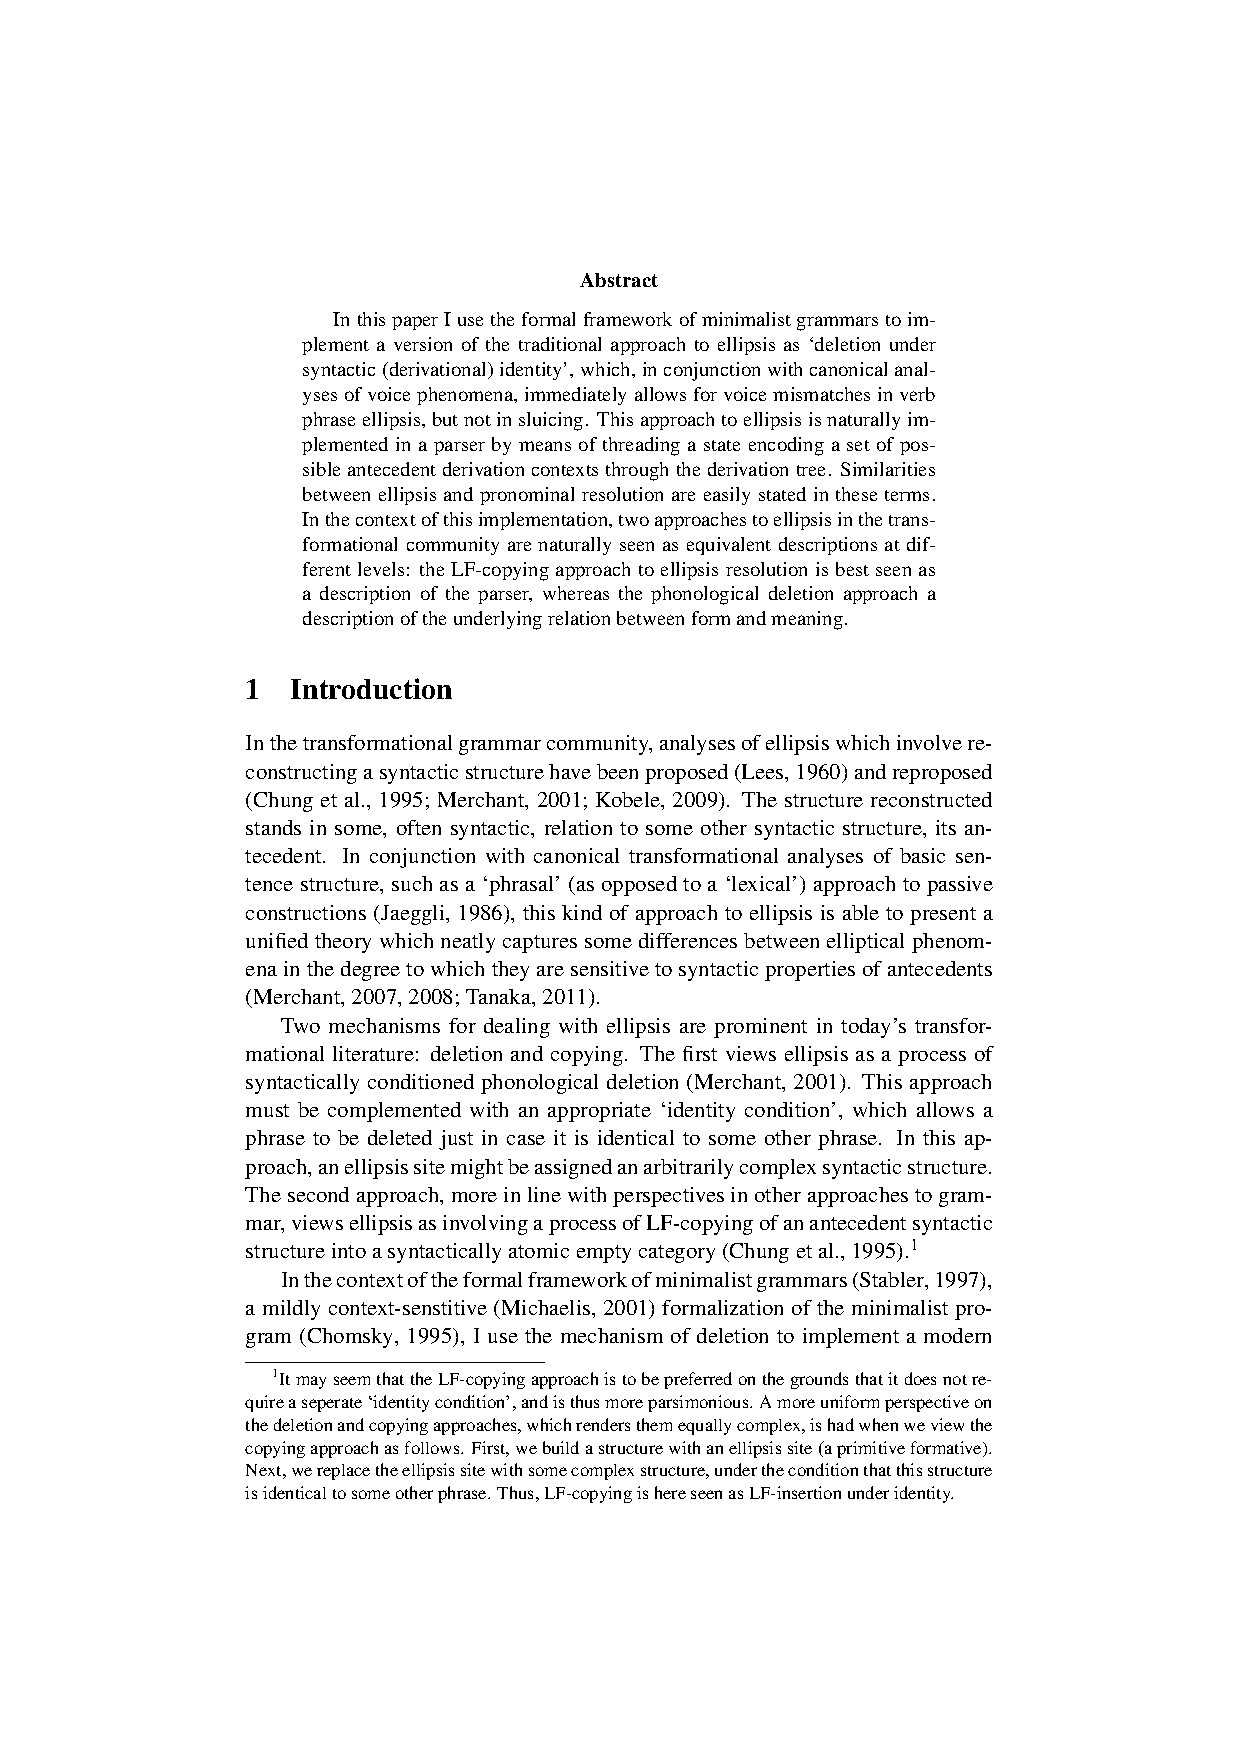
\includepdf[pages=-,pagecommand=\thispagestyle{plain}]{Includes/kobele.pdf}
        \setcounter{page}{427}
        \phantomsection
        \addcontentsline{toc}{section}{Hanjung Lee, Nayoun Kim: Non-Canonical Word Order and Subject-Object Asymmetry in Korean Case Ellipsis}
\thispagestyle{empty}

\begin{center}
  {\huge\bfseries Non-Canonical Word Order and Subject-Object Asymmetry in Korean Case Ellipsis\par}

  \bigskip

~\\
\begingroup
\setlength{\leftskip}{0pt plus 1fill}
\setlength{\rightskip}{0pt plus 1fill}
\setlength{\parindent}{0pt}
\setlength{\parfillskip}{0pt}
  \formatauthor{Hanjung Lee}{\begin{tabular}{@{}c@{}}Sungkyunkwan University\end{tabular}}
\formatauthor{Nayoun Kim}{\begin{tabular}{@{}c@{}}Sungkyunkwan University\end{tabular}}

\par\endgroup

  \vspace*{8ex}

  Proceedings of the 19th International Conference on\par Head-Driven Phrase Structure Grammar

  \bigskip

  Chungnam National University Daejeon

  \medskip

  Stefan Müller (Editor)

  \medskip

  2012

  \medskip

  CSLI Publications

  \medskip

  pages 427--442

  \medskip

  \url{http://csli-publications.stanford.edu/HPSG/2012}
\end{center}
\vfill

\noindent



\vfill
\noindent
% APA Style
Lee, Hanjung, \& Kim, Nayoun. 2012. Non-Canonical Word Order and Subject-Object Asymmetry in Korean Case Ellipsis. In Müller, Stefan (Ed.), \emph{{Proceedings of the 19th International Conference on Head-Driven Phrase Structure Grammar, Chungnam National University Daejeon}}, 427--442. Stanford,
CA: CSLI Publications. \hfill\href{http://creativecommons.org/licenses/by/4.0/}{\includegraphics[height=.75em]{Includes/ccby.eps}}

\newpage
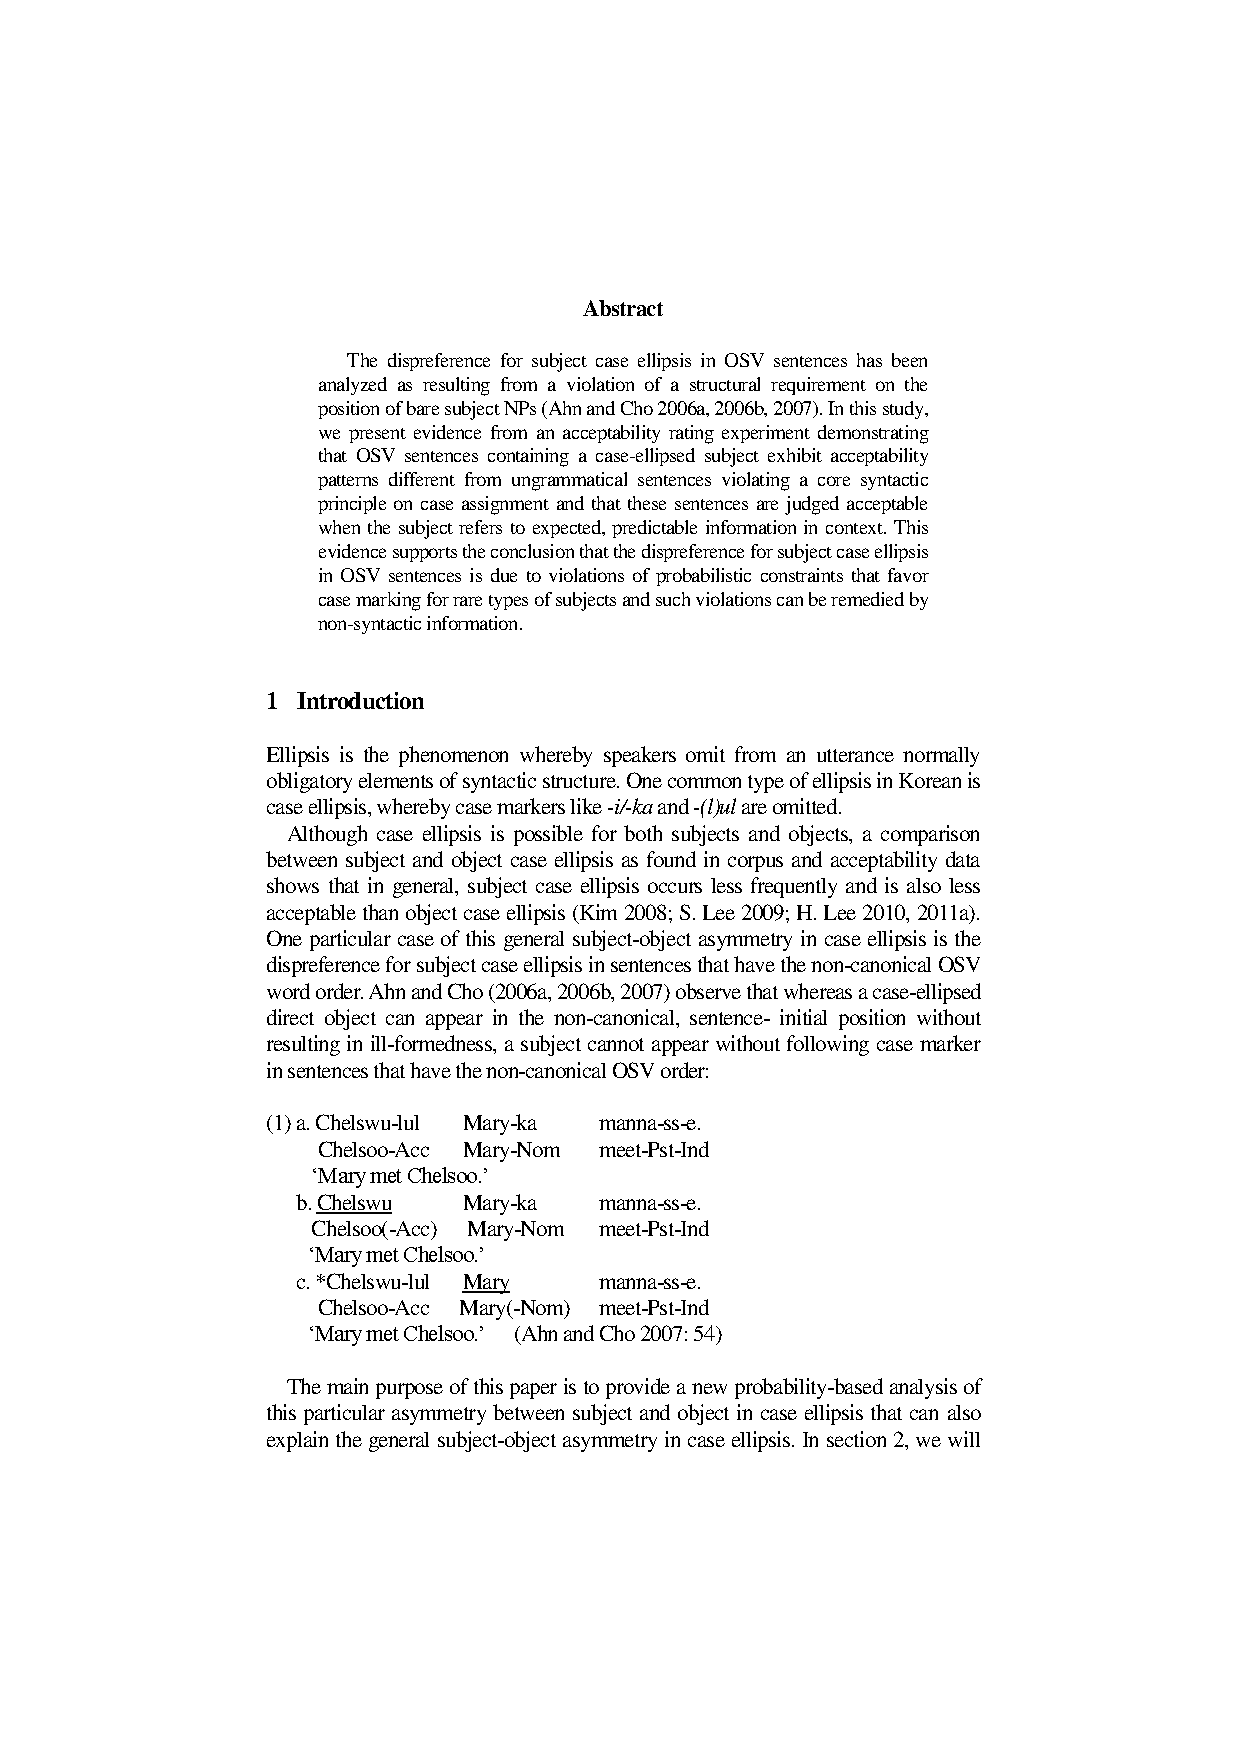
\includepdf[pages=-,pagecommand=\thispagestyle{plain}]{Includes/lee-kim.pdf}
        \setcounter{page}{443}
        \phantomsection
        \addcontentsline{toc}{section}{Yo Sato, Wai Lok Tam: Ellipsis of Case-Markers and Information Structure in Japanese}
\thispagestyle{empty}

\begin{center}
  {\huge\bfseries Ellipsis of Case-Markers and Information Structure in Japanese\par}

  \bigskip

~\\
\begingroup
\setlength{\leftskip}{0pt plus 1fill}
\setlength{\rightskip}{0pt plus 1fill}
\setlength{\parindent}{0pt}
\setlength{\parfillskip}{0pt}
  \formatauthor{Yo Sato}{\begin{tabular}{@{}c@{}}Department of Computer Science University of Hertfordshire\end{tabular}}
\formatauthor{Wai Lok Tam}{\begin{tabular}{@{}c@{}}National Institute of Advanced Industrial Science and Technology\end{tabular}}

\par\endgroup

  \vspace*{8ex}

  Proceedings of the 19th International Conference on\par Head-Driven Phrase Structure Grammar

  \bigskip

  Chungnam National University Daejeon

  \medskip

  Stefan Müller (Editor)

  \medskip

  2012

  \medskip

  CSLI Publications

  \medskip

  pages 443--453

  \medskip

  \url{http://csli-publications.stanford.edu/HPSG/2012}
\end{center}
\vfill

\noindent



\vfill
\noindent
% APA Style
Sato, Yo, \& Tam, Wai Lok. 2012. Ellipsis of Case-Markers and Information Structure in Japanese. In Müller, Stefan (Ed.), \emph{{Proceedings of the 19th International Conference on Head-Driven Phrase Structure Grammar, Chungnam National University Daejeon}}, 443--453. Stanford,
CA: CSLI Publications. \hfill\href{http://creativecommons.org/licenses/by/4.0/}{\includegraphics[height=.75em]{Includes/ccby.eps}}

\newpage
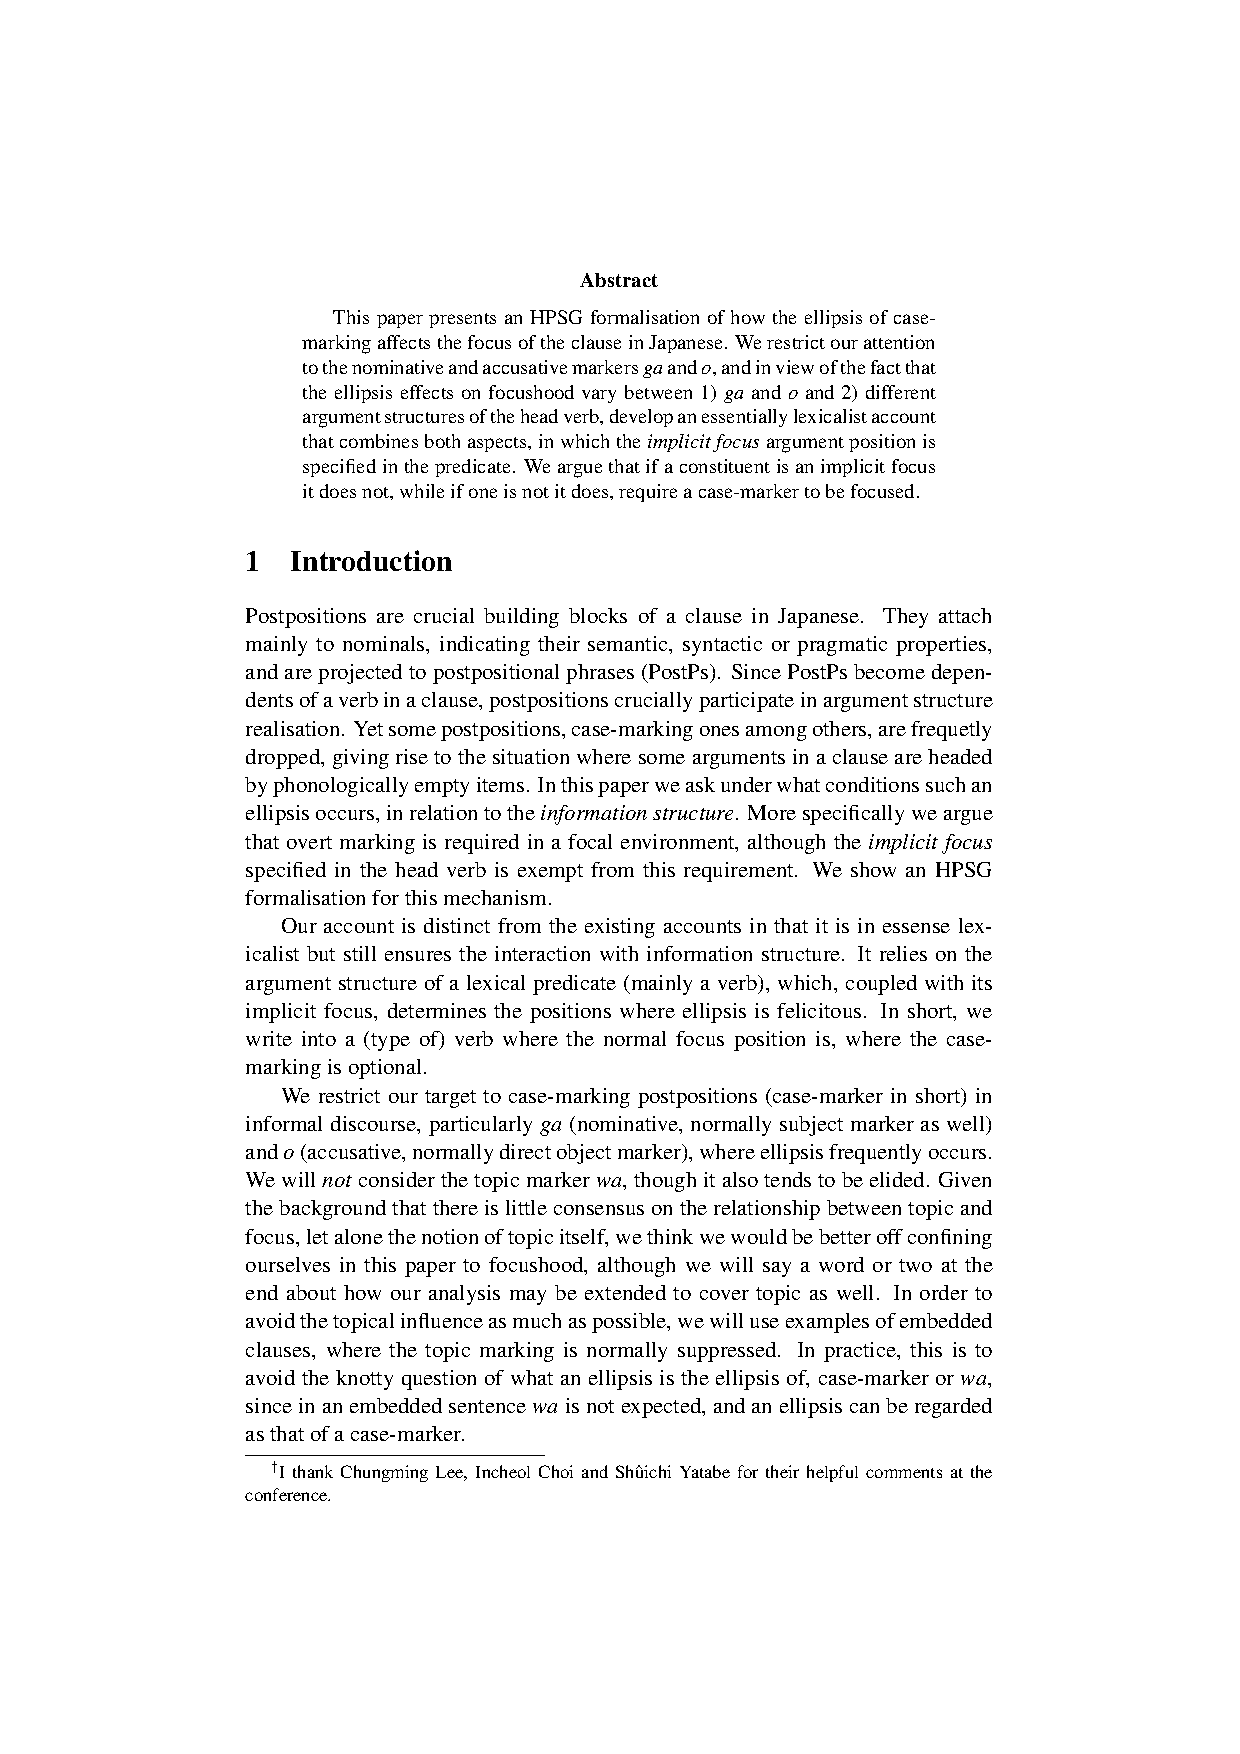
\includepdf[pages=-,pagecommand=\thispagestyle{plain}]{Includes/sato-tam.pdf}
        \setcounter{page}{454}
        \phantomsection
        \addcontentsline{toc}{section}{Sh{\^u}ichi Yatabe: Comparison of the Ellipsis-Based Theory of Non-Constituent Coordination with its Alternatives}
\thispagestyle{empty}

\begin{center}
  {\huge\bfseries Comparison of the Ellipsis-Based Theory of Non-Constituent Coordination with its Alternatives\par}

  \bigskip

~\\
\begingroup
\setlength{\leftskip}{0pt plus 1fill}
\setlength{\rightskip}{0pt plus 1fill}
\setlength{\parindent}{0pt}
\setlength{\parfillskip}{0pt}
  \formatauthor{Shûichi Yatabe}{\begin{tabular}{@{}c@{}}University of Tokyo\end{tabular}}

\par\endgroup

  \vspace*{8ex}

  Proceedings of the 19th International Conference on\par Head-Driven Phrase Structure Grammar

  \bigskip

  Chungnam National University Daejeon

  \medskip

  Stefan Müller (Editor)

  \medskip

  2012

  \medskip

  CSLI Publications

  \medskip

  pages 454--474

  \medskip

  \url{http://csli-publications.stanford.edu/HPSG/2012}
\end{center}
\vfill

\noindent



\vfill
\noindent
% APA Style
Yatabe, Shûichi. 2012. Comparison of the Ellipsis-Based Theory of Non-Constituent Coordination with its Alternatives. In Müller, Stefan (Ed.), \emph{{Proceedings of the 19th International Conference on Head-Driven Phrase Structure Grammar, Chungnam National University Daejeon}}, 454--474. Stanford,
CA: CSLI Publications. \hfill\href{http://creativecommons.org/licenses/by/4.0/}{\includegraphics[height=.75em]{Includes/ccby.eps}}

\newpage
\includepdf[pages=-,pagecommand=\thispagestyle{plain}]{Includes/yatabe.pdf}
\end{document}
